\documentclass{article}
%------------------------- packages -------------------------%
\usepackage[T1]{fontenc}
\usepackage[utf8]{vietnam}
\usepackage[unicode,hidelinks]{hyperref}    % for reference
\usepackage{geometry}   % for layout
\usepackage{amsmath}    % for math
\usepackage{xcolor}     % for color
% for figure
\usepackage{subcaption}
\usepackage{graphicx}
\usepackage{caption}    
% for code
\usepackage{minted}
\usepackage[normalem]{ulem}
% for table
\usepackage{float}      
\usepackage{paracol}
\usepackage{array}
\usepackage{multirow}
\usepackage{amssymb}
% for header & footer 
\usepackage{fancyhdr}
\usepackage{lastpage}
%\usepackage{CJKutf8}
\usepackage[most]{tcolorbox}
\tcbuselibrary{listings, skins, breakable}
\usepackage{listings}
\usepackage{tabularx}
\definecolor{dkgreen}{rgb}{0,0.6,0}
\definecolor{gray}{rgb}{0.5,0.5,0.5}
\definecolor{mauve}{rgb}{0.58,0,0.82}

% Cấu hình python trong latex
\newtcblisting{pythoncode}{
    breakable,
    boxrule=0pt,
    frame hidden,
    colback=gray!6!white,
    arc=2mm,
    top=2mm, bottom=2mm, left=2mm, right=2mm,
    listing only,
    listing options={
        language=Python,
        basicstyle=\ttfamily\footnotesize,
        keywordstyle=\color{blue}\bfseries,
        commentstyle=\color{dkgreen}\itshape,
        stringstyle=\color{mauve},
        breaklines=true,
        showstringspaces=false,
        tabsize=4,
        inputencoding=utf8,
        extendedchars=true
    }
}

% Cách dùng trong bài:
%\begin{pythoncode}{Giai đoạn 1: Trích lọc tập biến quan tâm}
%import pandas as pd
%df_raw = pd.read_csv('data/All_GPUs.csv')
%\end{pythoncode}

\lstset{frame=tb,
    language=Python,
    aboveskip=3mm,
    belowskip=3mm,
    showstringspaces=false,
    columns=flexible,
    basicstyle={\small\ttfamily},
    numbers=none,
    numberstyle=\tiny\color{gray},
    keywordstyle=\color{blue},
    commentstyle=\color{dkgreen},
    stringstyle=\color{mauve},
    breaklines=true,
    breakatwhitespace=true,
    tabsize=3,
}

%------------------------- set up -------------------------%
% figure
\graphicspath{{./img/}}              % path to image
\captionsetup[figure]{labelfont={small,bf,it},textfont={small,it}}
% paragraph
\setlength{\parindent}{0pt}
\setlength{\parskip}{6pt}               % disables indentation
\renewcommand{\baselinestretch}{1.5}    % line spacing
% color
\definecolor{codegreen}{rgb}{0,0.6,0}
\definecolor{codegray}{rgb}{0.5,0.5,0.5}
\definecolor{codepurple}{rgb}{0.58,0,0.82}
% code
\def\code#1{\texttt{#1}}    % font
\usemintedstyle{vs}         % minted theme
\setminted{
    autogobble,             % remove all common leading whitespace
    baselinestretch=1.0,
    bgcolor=gray!5!white,
    breaklines,
    %linenos,               % enables line numbers
    fontsize=\footnotesize
}

%------------------------- layout & margin -------------------------%
\geometry{
    a4paper,        % redundant if already in \documentclass
    left=20.32mm,
    right=20.32mm,
    top=25.40mm,
    bottom=25.40mm,
    heightrounded,  % better use it
}

%------------------------- header & footer -------------------------%
\renewcommand{\headrulewidth}{0.5pt}
\renewcommand{\footrulewidth}{0.5pt}
\setlength{\headheight}{24.5pt}
\pagestyle{fancy}

\fancyhead{}    % clear all header fields
\fancyhead[L]{
    \begin{tabular}{ll}
        \begin{picture}(10,10)
            \put(0,-7){
\includegraphics[width=8mm]{hcmut_logo.png}}
        \end{picture}&
    	\begin{tabular}{l}
    	    {\ttfamily Trường Đại học Bách Khoa Tp. Hồ Chí Minh} \\
    	    {\ttfamily Khoa Khoa học và Kỹ thuật Máy tính} \\
    	\end{tabular} 	
    \end{tabular}
}

\fancyfoot{}    % clear all footer fields
\fancyfoot[L]{\footnotesize {\ttfamily Báo cáo BTL Xác suất thống kê}}
\fancyfoot[R]{\footnotesize {\ttfamily Trang {\thepage}/\pageref{LastPage}}}
% might change to \scriptsize


% addtional fix
%------------------------- body -------------------------%
\begin{document}

%-------------------- cover --------------------%
\begin{titlepage}
\begin{center}
    \large ĐẠI HỌC QUỐC GIA THÀNH PHỐ HỒ CHÍ MINH \\
    TRƯỜNG ĐẠI HỌC BÁCH KHOA \\
    KHOA KHOA HỌC VÀ KỸ THUẬT MÁY TÍNH
\end{center}

\vspace{1.5cm}

\begin{figure}[!ht]
    \centering 
\includegraphics[width=3.5cm]{hcmut_logo.png}
\end{figure}

\vspace{1.5cm}

\begin{table}[H]
    \centering
    \begin{tabular}{c}
    {\bf \Large XÁC SUẤT THỐNG KÊ} \\ \\
    \hline  \\
    \multicolumn{1}{l}{{\bf \large Bài tập lớn}}    \\  \\
    {\bf \huge TỔNG QUAN VỀ HIỆU NĂNG }     \\  
    
    \hline
    \end{tabular}
\end{table}

\vspace{1.5cm}

\begin{table}[H]
\centering
\begin{tabular}{lrlc}
\hspace{5.5 cm} & Giảng viên hướng dẫn: & Nguyễn Đình Huy   & \\
                & Sinh viên thực hiện:  & Võ Huỳnh Anh Thư    & 2213416 \\
                &   &  &  \\
                &   &   & \\
                &   &  & \\
                
        
\end{tabular}
\textbf{\textit{}}\end{table}

\vspace{1.0cm}

\begin{center}
    \footnotesize Tp. Hồ Chí Minh, Tháng 10/2026
\end{center}
\end{titlepage}

\newpage
%-------------------- mission --------------------%
%\renewcommand{\arraystretch}{2}

%-------------------- contents --------------------%
\tableofcontents
\newpage
\section{Danh sách thành viên \& Khối lượng công việc}
\begin{table}[htbp]
    \centering
    \renewcommand{\arraystretch}{1.8} % Tăng khoảng cách dòng tạo độ thoáng như hình
    \begin{tabularx}{\textwidth}{|>{\centering\arraybackslash}m{1.2cm}|>{\centering\arraybackslash}m{4.2cm}|>{\centering\arraybackslash}m{2cm}|>{\raggedright\arraybackslash}X|>{\centering\arraybackslash}m{3.8cm}|}
        \hline
        \textbf{STT} & \textbf{Họ và tên} & \textbf{MSSV} & \textbf{Phân công công việc} & \textbf{Mức độ hoàn thành} \\
        \hline
        1 &  &  & - Xử lí số liệu \newline
        - Code & 20\% \\
        \hline
        2 &  &  & - Xử lí số liệu \newline 
        - Code & 20\% \\
        \hline
        3 &  &  & - Thống kê mô tả \newline
        - Thống kê suy diễn (Phần 6.1, 6.2) & 20\% \\
        \hline
        4 &  &  & - Thống kê suy diễn (Phần 6.3, 6.4, 6.5) & 20\% \\
        \hline
        5 &  &  & - Kiến thức nền & 20\% \\
        \hline
    \end{tabularx}
\end{table}
\newpage
\section{Tổng quan dữ liệu}
\newpage
\section{Kiến thức nền}
\subsection{Phân tích và khám phá dữ liệu}
\subsection{Hồi quy tuyến tính bội}
\subsection{Độ phù hợp của mô hình}
\subsection{Lý thuyết về ANOVA (Phân tích phương sai)}
\newpage
\section{Tiền xử lý số liệu}
    Trong phần Tiền xử lý dữ liệu, nhóm sử dụng môi trường lập trình \textbf{R} và giao diện \textbf{RStudio} làm công cụ xử lý dữ liệu gốc. Để chuẩn bị dữ liệu đầu vào chuẩn xác và có độ tin cậy cao cho các phân tích thống kê mô tả cũng như hồi quy tuyến tính ở các phần sau, nhóm tiến hành quy trình tiền xử lý dữ liệu qua 4 giai đoạn cụ thể dưới đây.

    \subsection{Trích lọc tập biến quan tâm}
        Bộ dữ liệu ban đầu \texttt{All\_GPUs.csv} gồm 3,406 mẫu quan sát và 34 biến thông số kỹ thuật. Nhóm lọc ra 9 thông số kỹ thuật phần cứng cốt lõi nhất đại diện cho năng lực xử lý nhân và hệ thống bộ nhớ GPU, đồng thời giữ lại biến định danh tên sản phẩm (\texttt{Name}) để phục vụ bước lọc trùng lặp:

        \begin{itemize}
            \item \textbf{Biến định danh}: \texttt{Name} (Tên mẫu card đồ họa).
            \item \textbf{Biến nhân xử lý}: \texttt{Core\_Speed} (MHz), \texttt{Max\_Power} (Watts), \texttt{Process} (nm), \texttt{ROPs}, \texttt{TMUs}.
            \item \textbf{Biến hệ thống bộ nhớ}: \texttt{Memory} (MB), \texttt{Memory\_Bandwidth} (GB/s), \texttt{Memory\_Bus} (Bit), \texttt{Memory\_Speed} (MHz).
        \end{itemize}

        Đọc dữ liệu bằng hàm \texttt{read.csv()} của R, chuẩn hóa các chuỗi đại diện cho dữ liệu khuyết như \texttt{"\textbackslash n-"}, \texttt{"-"}, \texttt{"None"}, \texttt{""} thành \texttt{NA}.

        \begin{figure}[H]
            \centering
            \begin{subfigure}[b]{0.92\textwidth}
                \centering
                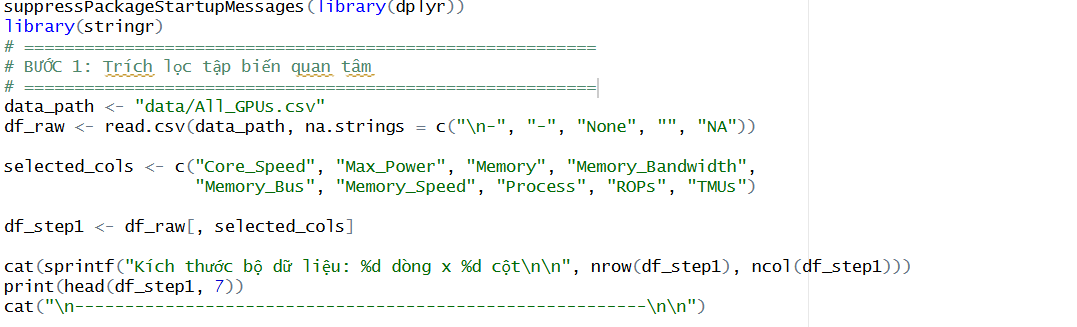
\includegraphics[width=\textwidth]{dataPrep/m1a.png}
            \end{subfigure}
            \vspace{0.4cm}
            \begin{subfigure}[b]{0.92\textwidth}
                \centering
                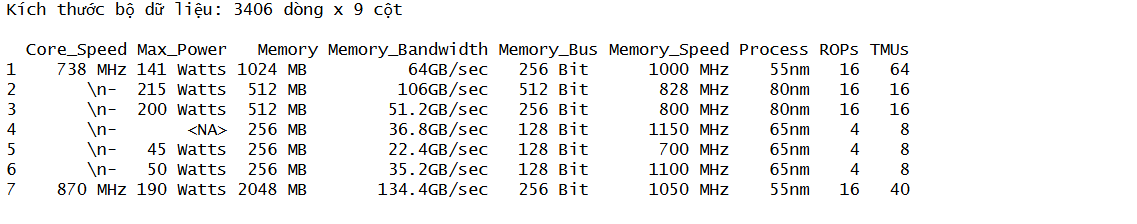
\includegraphics[width=\textwidth]{dataPrep/m1b.png}
            \end{subfigure}
            \caption{Kết quả trích lọc tập biến quan tâm}
            \label{fig:Trích lọc tập biến quan tâm}
        \end{figure}

    \subsection{Tách bỏ đơn vị, quy đổi hệ số và chuyển đổi kiểu dữ liệu}
        Dữ liệu gốc chứa các ký tự đơn vị và hậu tố đi kèm. Nhóm sử dụng thư viện \texttt{stringr} để trích xuất giá trị số thực và chuẩn hóa đồng nhất đơn vị cho toàn bộ 9 cột về kiểu dữ liệu số (\texttt{numeric}):
        \begin{itemize}
            \item \textbf{Chuẩn hóa băng thông (\texttt{Memory\_Bandwidth}):} Một số dòng GPU đời cũ sử dụng đơn vị \texttt{MB/sec} thay vì \texttt{GB/sec}. Nhóm thực hiện nhận diện chuỗi \texttt{"MB"} và chia cho $1024$ để quy đổi toàn bộ cột về chung đơn vị chuẩn \texttt{GB/sec}.
            \item \textbf{Xử lý hậu tố nhân đơn vị (\texttt{ROPs}, \texttt{TMUs}):} Các cấu hình GPU nhân đôi (Dual-GPU) có giá trị dạng \texttt{16 (x2)}. Hệ thống tự động tách phần số gốc và nhân với hệ số trong ngoặc (ví dụ: $16 \times 2 = 32$) để phản ánh đúng tổng năng lực phần cứng thực tế.
            \item \textbf{Các biến còn lại:} Loại bỏ các hậu tố \texttt{MHz}, \texttt{Watts}, \texttt{MB}, \texttt{Bit}, \texttt{nm} và ép kiểu sang \texttt{numeric}.
        \end{itemize}

        \begin{figure}[H]
            \centering
            \begin{subfigure}[b]{0.92\textwidth}
                \centering
                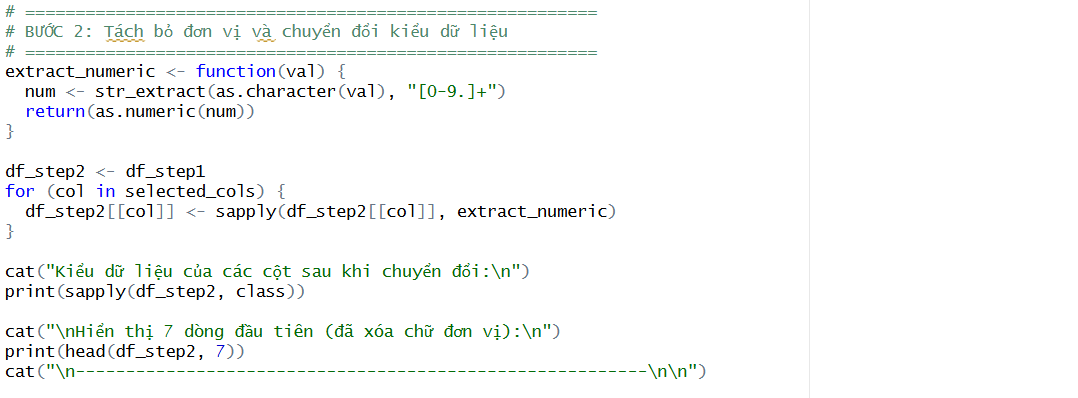
\includegraphics[width=\textwidth]{dataPrep/m2a.png}
            \end{subfigure}
            \vspace{0.4cm}
            \begin{subfigure}[b]{0.92\textwidth}
                \centering
                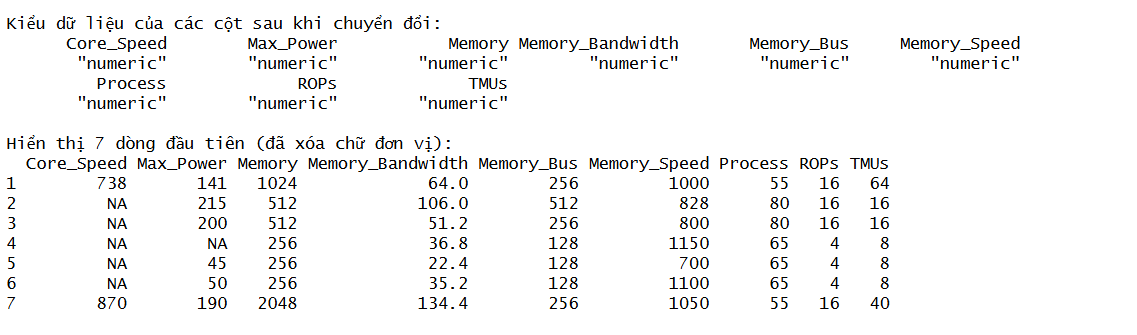
\includegraphics[width=\textwidth]{dataPrep/m2b.png}
            \end{subfigure}
            \caption{Kết quả tách bỏ đơn vị và chuyển đổi kiểu dữ liệu}
            \label{fig:Tách bỏ đơn vị và chuyển đổi kiểu dữ liệu}
        \end{figure}

    \subsection{Chuẩn hóa ô trống và xử lý dữ liệu khuyết}
        Dữ liệu khuyết trong tập dữ liệu mang đặc tính không hoàn toàn ngẫu nhiên (MAR/MNAR) do các dòng GPU đời cũ hoặc chip tích hợp thường không công bố đầy đủ thông số. Do các thông số phần cứng mang tính kiến trúc cố định, việc thay thế dữ liệu (Imputation) bằng giá trị trung bình/trung vị có thể làm bóp méo bản chất kỹ thuật. Nhóm áp dụng phương pháp \textbf{Loại bỏ theo dòng (Listwise Deletion)} bằng hàm \texttt{na.omit()}.

        \begin{figure}[H]
            \centering
            \begin{subfigure}[b]{0.92\textwidth}
                \centering
                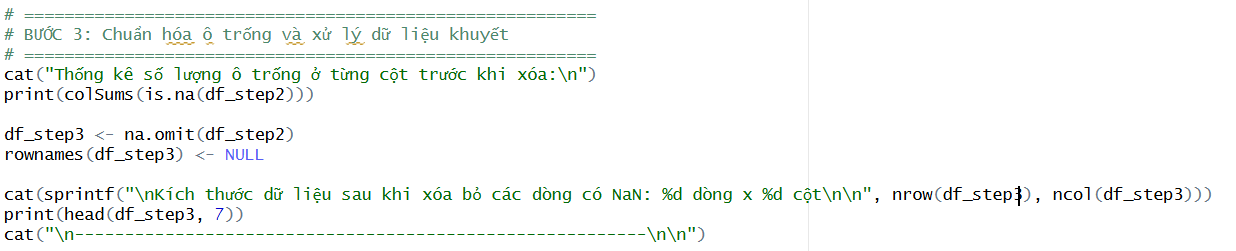
\includegraphics[width=\textwidth]{dataPrep/m3a.png}
            \end{subfigure}
            \vspace{0.4cm}
            \begin{subfigure}[b]{0.92\textwidth}
                \centering
                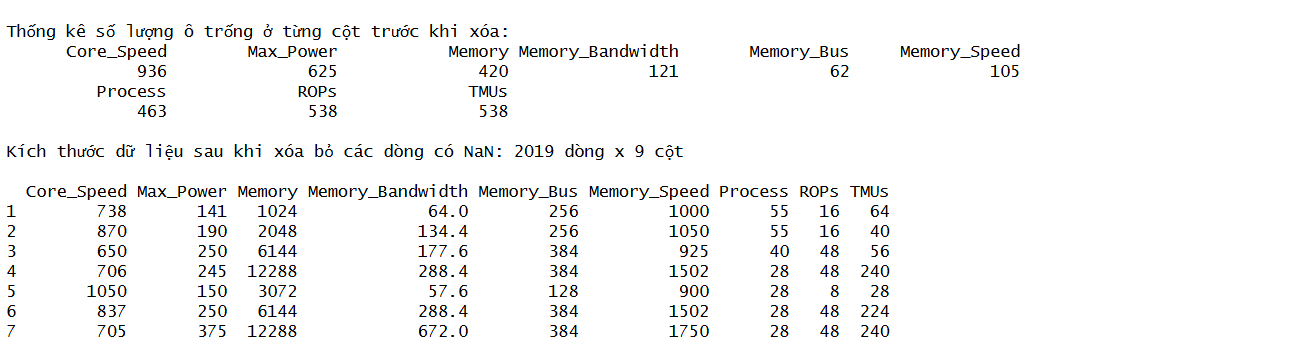
\includegraphics[width=\textwidth]{dataPrep/m3b.png}
            \end{subfigure}
            \caption{Kết quả thống kê ô trống và loại bỏ dữ liệu khuyết}
            \label{fig: Chuẩn hóa ô trống và xử lý dữ liệu khuyết}
        \end{figure}

    \subsection{Loại bỏ quan sát trùng lặp theo từng mẫu GPU}
        Trong thực tế phần cứng, hai mẫu card đồ họa khác tên (ví dụ các phiên bản thương mại khác nhau hoặc khác dòng sản phẩm) vẫn có thể sở hữu bộ 9 thông số kỹ thuật giống nhau. Nếu lọc trùng dựa trên 9 thông số sẽ vô tình làm mất đi các quan sát hợp lệ. Do đó, nhóm thực hiện lọc trùng dựa trên biến định danh tên sản phẩm (\texttt{Name}) bằng hàm \texttt{distinct(Name, .keep\_all = TRUE)} thuộc gói \texttt{dplyr} để đảm bảo mỗi dòng đại diện cho một mẫu GPU duy nhất, sau đó mới loại bỏ cột \texttt{Name} để thu được bảng dữ liệu định lượng sạch hoàn chỉnh.

        \begin{figure}[H]
            \centering
            \begin{subfigure}[b]{0.92\textwidth}
                \centering
                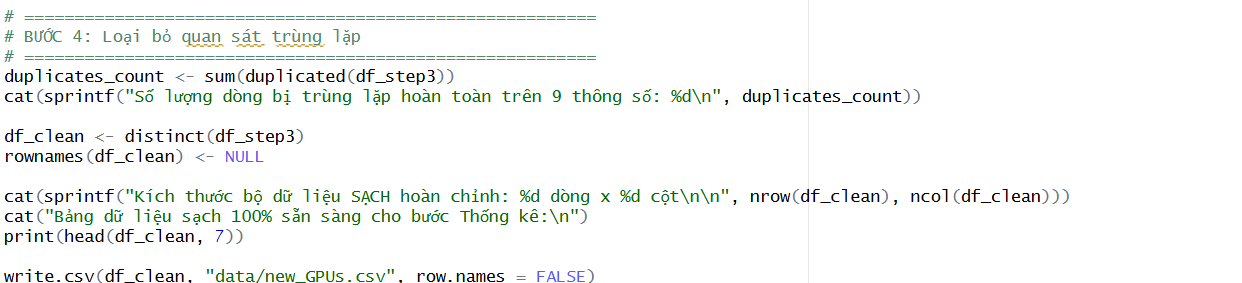
\includegraphics[width=\textwidth]{dataPrep/m4a.png}
            \end{subfigure}
            \vspace{0.4cm}
            \begin{subfigure}[b]{0.92\textwidth}
                \centering
                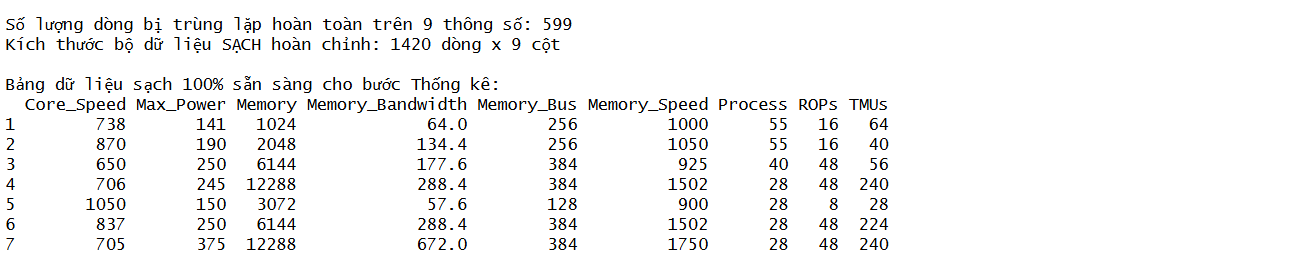
\includegraphics[width=\textwidth]{dataPrep/m4b.png}
            \end{subfigure}
            \caption{Kết quả loại bỏ quan sát trùng lặp theo tên GPU}
            \label{fig:Loại bỏ quan sát trùng lặp}
        \end{figure}

    \subsection{Mã nguồn xử lý bằng R}
        Đoạn mã R thực hiện trọn vẹn 4 giai đoạn tiền xử lý:

\begin{pythoncode}
suppressPackageStartupMessages(library(dplyr))
library(stringr)

# BUOC 1: Trich loc 9 bien quan tam kem bien dinh danh Name
df_raw <- read.csv('data/All_GPUs.csv', na.strings = c('\n-', '-', 'None', '', 'NA'))
selected_cols <- c('Core_Speed', 'Max_Power', 'Memory', 'Memory_Bandwidth', 
                   'Memory_Bus', 'Memory_Speed', 'Process', 'ROPs', 'TMUs')
df_step1 <- df_raw[, c('Name', selected_cols)]

# BUOC 2: Tach don vi, quy doi MB/s -> GB/s va nhan he so (x2)
extract_numeric <- function(val) as.numeric(str_extract(as.character(val), '[0-9.]+'))

parse_bandwidth <- function(val) {
  str_val <- as.character(val)
  num <- as.numeric(str_extract(str_val, '[0-9.]+'))
  is_mb <- str_detect(str_val, regex('MB', ignore_case = TRUE))
  ifelse(!is.na(num) & !is.na(is_mb) & is_mb, num / 1024, num)
}

parse_units_multiplier <- function(val) {
  str_val <- as.character(val)
  base_num <- as.numeric(str_extract(str_val, '^[0-9.]+'))
  mult_str <- str_extract(str_val, '(?<=\\(x)[0-9.]+(?=\\))')
  mult <- ifelse(is.na(mult_str), 1, as.numeric(mult_str))
  return(base_num * mult)
}

df_step2 <- df_step1
for (col in selected_cols) {
  if (col == 'Memory_Bandwidth') {
    df_step2[[col]] <- parse_bandwidth(df_step2[[col]])
  } else if (col %in% c('ROPs', 'TMUs')) {
    df_step2[[col]] <- parse_units_multiplier(df_step2[[col]])
  } else {
    df_step2[[col]] <- sapply(df_step2[[col]], extract_numeric)
  }
}

# BUOC 3: Xu ly du lieu khuyet (Listwise Deletion)
df_step3 <- na.omit(df_step2)

# BUOC 4: Loai bo trung lap theo ten mau GPU (Name)
df_step3$Name <- str_trim(as.character(df_step3$Name))
df_clean <- df_step3 %>%
  distinct(Name, .keep_all = TRUE) %>%
  select(all_of(selected_cols))

write.csv(df_clean, 'data/new_GPUs.csv', row.names = FALSE)
\end{pythoncode}
\newpage
\section{Thống kê mô tả}

    \subsection{Thông tin tổng quát về các biến của bộ dữ liệu}
        Bộ dữ liệu sau khi tiền xử lý bao gồm 9 thông số kỹ thuật phần cứng cốt lõi ảnh hưởng đến hiệu năng của GPU. Dưới đây là bảng mô tả chi tiết kiểu biến, đơn vị đo lường và ý nghĩa của các biến chính:

        \begin{table}[H]
            \centering
            \renewcommand{\arraystretch}{1.3}
            \begin{tabular}{|l|l|c|p{6.2cm}|}
                \hline
                \textbf{Tên biến} & \textbf{Kiểu biến} & \textbf{Đơn vị} & \textbf{Mô tả \& Ý nghĩa} \\
                \hline
                \texttt{Core\_Speed} & Liên tục & MHz & Tốc độ xử lý xung nhịp của GPU, thể hiện số chu kỳ thực hiện được trong 1 giây. \\
                \hline
                \texttt{Memory} & Liên tục & MB & Dung lượng bộ nhớ VRAM của GPU, dùng để lưu trữ dữ liệu và tài nguyên đồ họa. \\
                \hline
                \texttt{Memory\_Bus} & Liên tục & Bit & Độ rộng kênh truyền dẫn dữ liệu giữa bộ nhớ VRAM và các nhân xử lý của GPU. \\
                \hline
                \texttt{Max\_Power} & Liên tục & W & Công suất tiêu thụ tối đa (TDP), thể hiện giới hạn năng lượng cung cấp cho card đồ họa. \\
                \hline
                \texttt{Memory\_Bandwidth} & Liên tục & GB/s & Băng thông bộ nhớ, thể hiện tốc độ truyền tải dữ liệu tối đa giữa GPU và bộ nhớ. \\
                \hline
                \texttt{Memory\_Speed} & Liên tục & MHz & Tốc độ xung nhịp hoạt động của bộ nhớ RAM trên GPU. \\
                \hline
                \texttt{Process} & Liên tục & nm & Tiến trình công nghệ bán dẫn (nanometer) sử dụng trong quá trình chế tạo chip GPU. \\
                \hline
                \texttt{ROPs} & Liên tục & Đơn vị & Số đơn vị xuất kết xuất (Raster Operations Pipelines), xử lý pixel cuối cùng trước khi xuất ra màn hình. \\
                \hline
                \texttt{TMUs} & Liên tục & Đơn vị & Số đơn vị ánh xạ vân bề mặt (Texture Mapping Units), chịu trách nhiệm xử lý và lọc texture. \\
                \hline
            \end{tabular}
            \caption{Thông tin tổng quát về các biến trong bộ dữ liệu GPU}
            \label{tab:thong_tin_bien}
        \end{table}

    \subsection{Bảng các đặc trưng thống kê mô tả}
        Để có cái nhìn định lượng tổng quan về xu hướng tập trung và mức độ phân tán của từng thông số kỹ thuật trước khi biến đổi logarit, nhóm tính toán các tham số thống kê mô tả cơ bản trên tập dữ liệu sạch (kết quả trích xuất từ tệp \texttt{summary\_stats.csv} sau khi chạy lại quy trình tiền xử lý mới):

        \begin{table}[H]
            \centering
            \footnotesize
            \renewcommand{\arraystretch}{1.35}
            \begin{tabular}{|l|c|r|r|r|r|r|r|r|r|}
                \hline
                \textbf{Tên biến} & \textbf{Đơn vị} & \textbf{$N$} & \textbf{Mean} & \textbf{SD} & \textbf{Min} & \textbf{$Q_1$} & \textbf{Median} & \textbf{$Q_3$} & \textbf{Max} \\
                \hline
                \texttt{Core\_Speed} & MHz & 2018 & 982.22 & 256.27 & 200.00 & 800.00 & 1000.00 & 1118.50 & 1784.00 \\
                \hline
                \texttt{Max\_Power} & W & 2018 & 143.36 & 103.73 & 1.00 & 65.00 & 122.00 & 190.00 & 780.00 \\
                \hline
                \texttt{Memory} & MB & 2018 & 3301.90 & 2762.80 & 128.00 & 1280.00 & 2048.00 & 4096.00 & 24576.00 \\
                \hline
                \texttt{Memory\_Bandwidth} & GB/s & 2018 & 164.69 & 137.63 & 4.00 & 70.80 & 128.00 & 224.40 & 1280.00 \\
                \hline
                \texttt{Memory\_Bus} & Bit & 2018 & 223.11 & 247.13 & 64.00 & 128.00 & 192.00 & 256.00 & 4096.00 \\
                \hline
                \texttt{Memory\_Speed} & MHz & 2018 & 1310.03 & 386.16 & 400.00 & 1000.00 & 1350.00 & 1653.00 & 2127.00 \\
                \hline
                \texttt{Process} & nm & 2018 & 30.18 & 10.49 & 14.00 & 28.00 & 28.00 & 40.00 & 90.00 \\
                \hline
                \texttt{ROPs} & Đơn vị & 2018 & 33.93 & 27.82 & 2.00 & 16.00 & 32.00 & 48.00 & 192.00 \\
                \hline
                \texttt{TMUs} & Đơn vị & 2018 & 76.73 & 55.61 & 4.00 & 32.00 & 64.00 & 112.00 & 384.00 \\
                \hline
            \end{tabular}
            \caption{Bảng các đặc trưng thống kê mô tả của 9 biến thông số kỹ thuật GPU}
            \label{tab:dac_trung_thong_ke}
        \end{table}

        \textbf{Nhận xét từ bảng số liệu:}
        \begin{itemize}
            \item Sự chênh lệch lớn giữa giá trị trung bình (\texttt{Mean}) và trung vị (\texttt{Median}), cùng với khoảng cách rất rộng từ tứ phân vị thứ ba ($Q_3$) đến giá trị cực đại (\texttt{Max}) ở các biến như \texttt{Memory}, \texttt{Memory\_Bandwidth}, \texttt{Max\_Power}, \texttt{ROPs}, và \texttt{TMUs} cho thấy dữ liệu có độ phân tán cao và bị lệch phải mạnh.
            \item Việc thực hiện phép chuyển đổi logarit ở bước tiếp theo là hoàn toàn cần thiết để thu hẹp khoảng biến thiên và giảm ảnh hưởng của các giá trị cực đại.
        \end{itemize}

    \subsection{Biểu đồ - đồ thị}
        \subsubsection{Biểu đồ phân bố tần suất (Histogram)}
            Dưới đây là biểu đồ phân bố tần suất cho các biến thông số kỹ thuật phần cứng của GPU trước và sau khi thực hiện phép biến đổi logarit (được vẽ bằng thư viện \texttt{ggplot2} và \texttt{gridExtra} trong R):

            \begin{figure}[H]
                \centering
                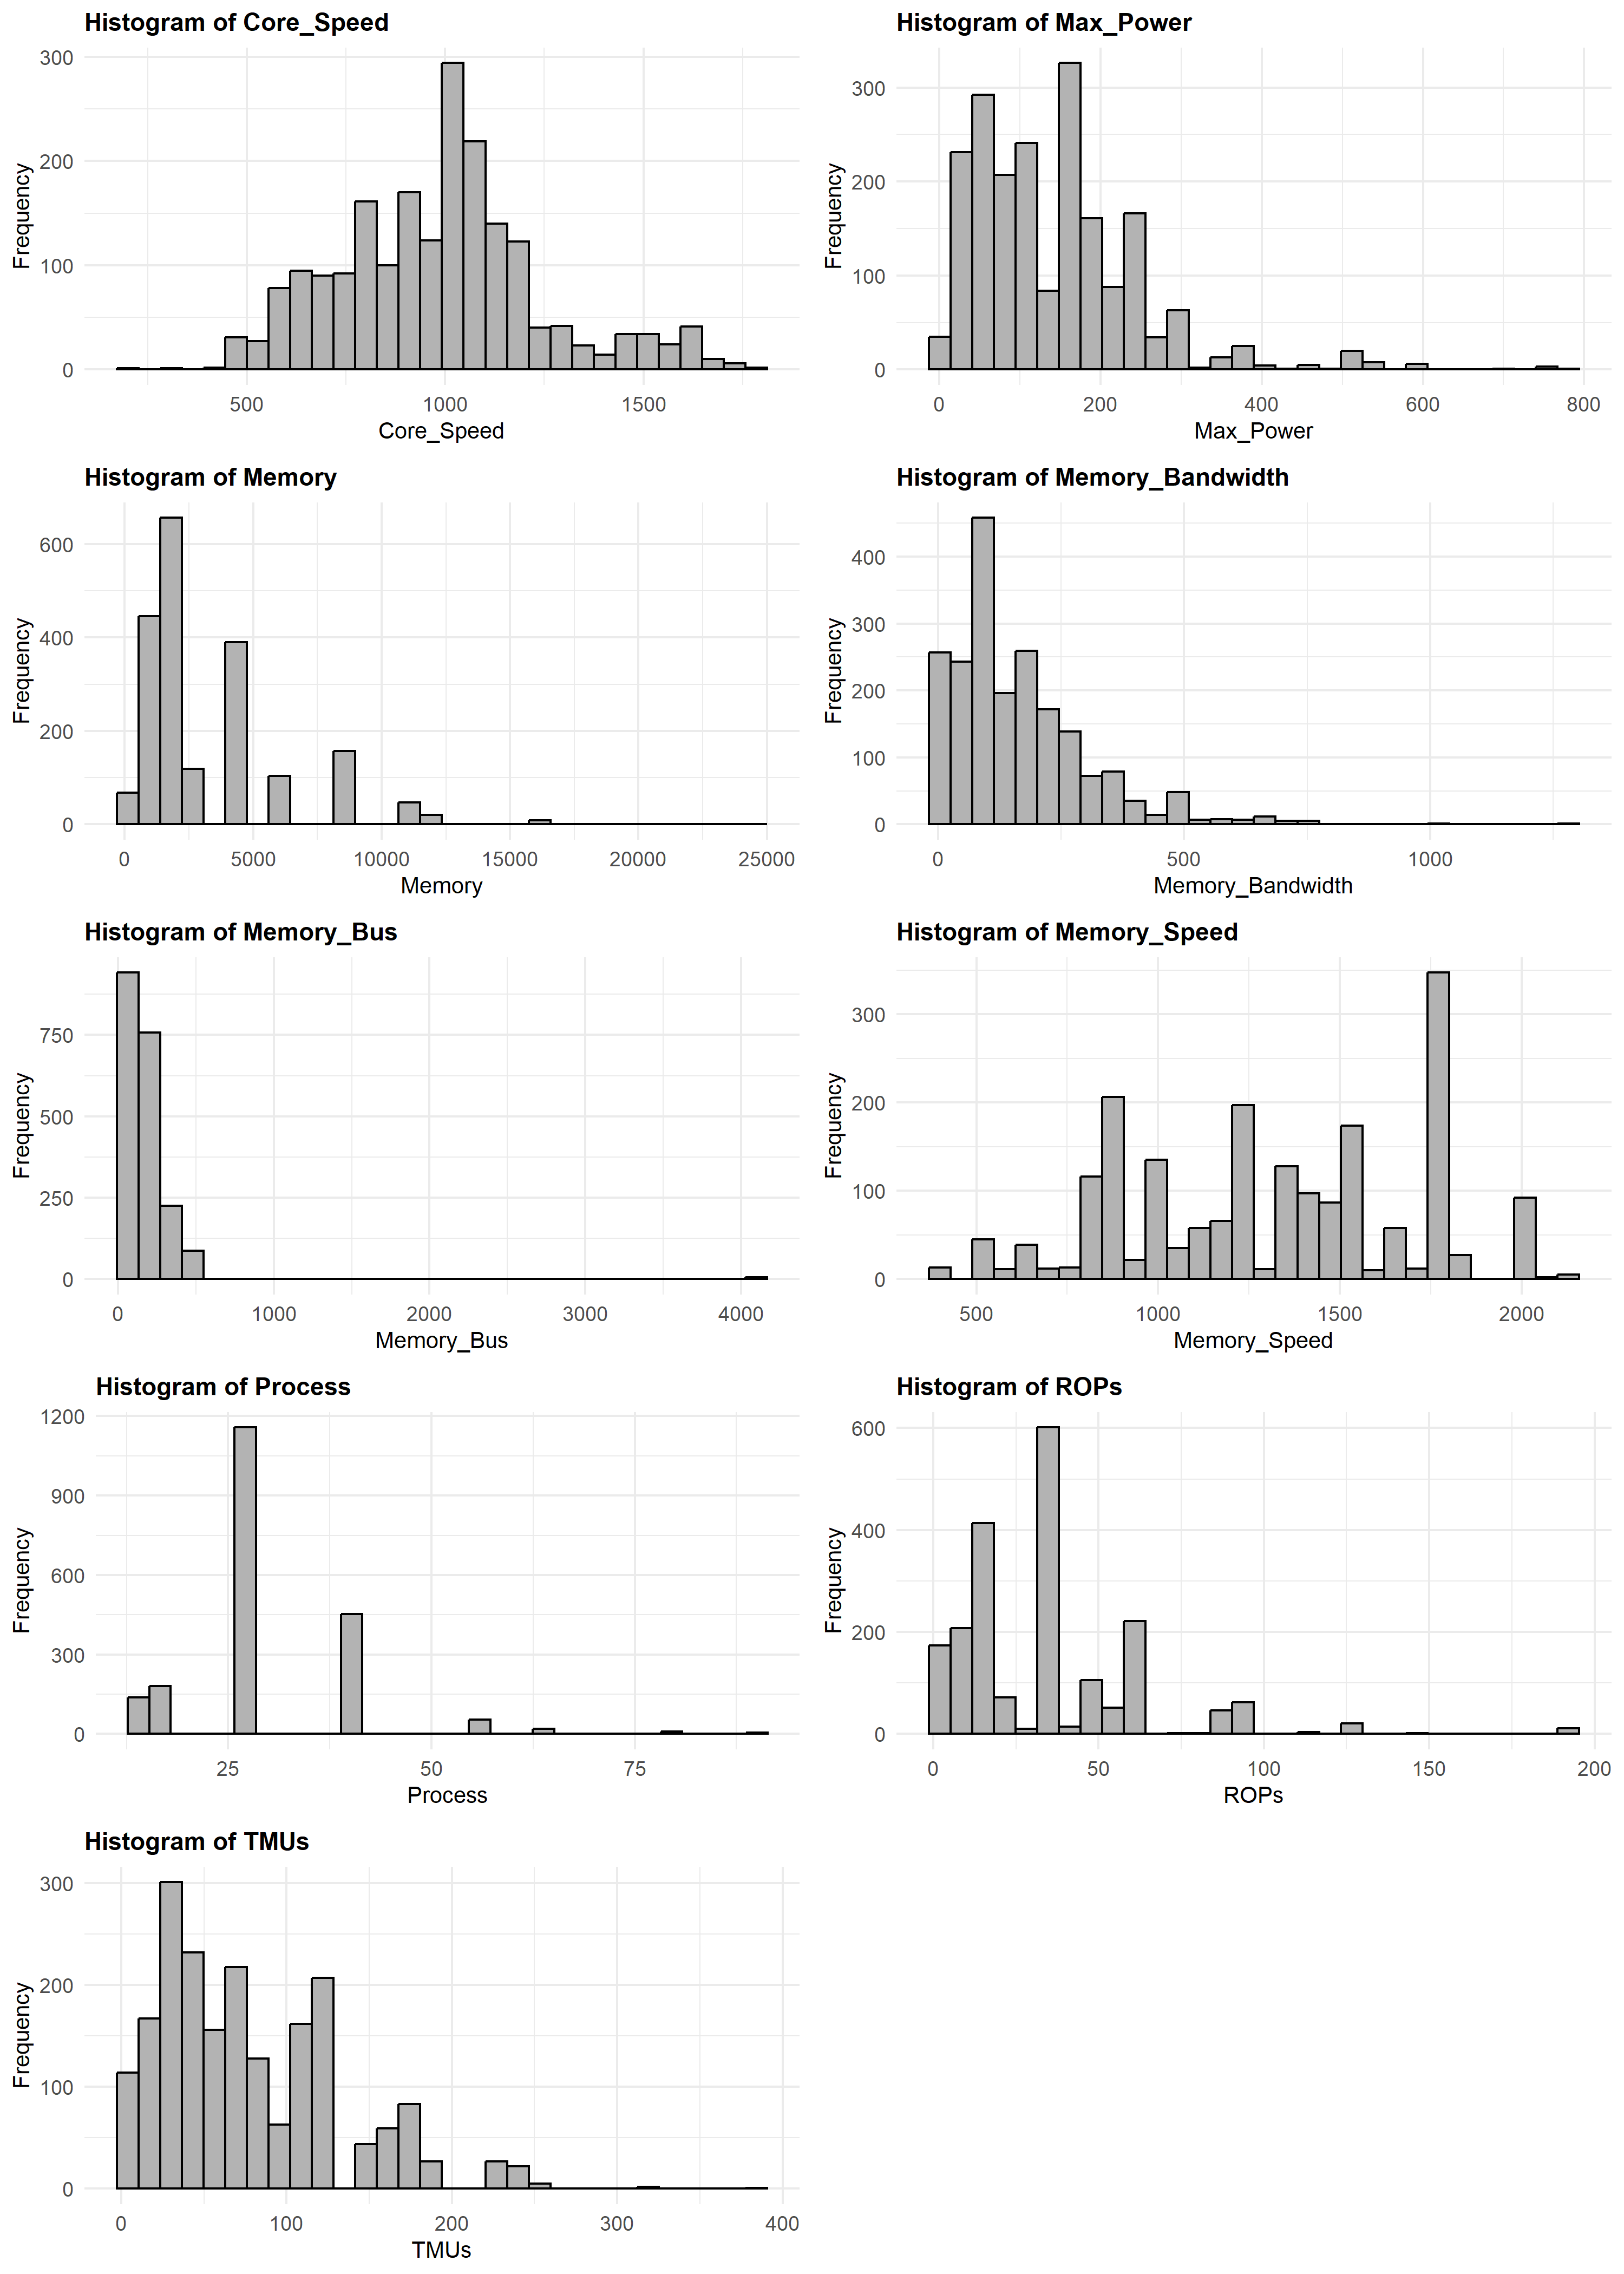
\includegraphics[width=0.92\textwidth]{statisticDes/histograms_original.png}
                \caption{Biểu đồ Histogram của các biến ở dạng dữ liệu gốc}
                \label{fig:hist_original_r5}
            \end{figure}

            \begin{figure}[H]
                \centering
                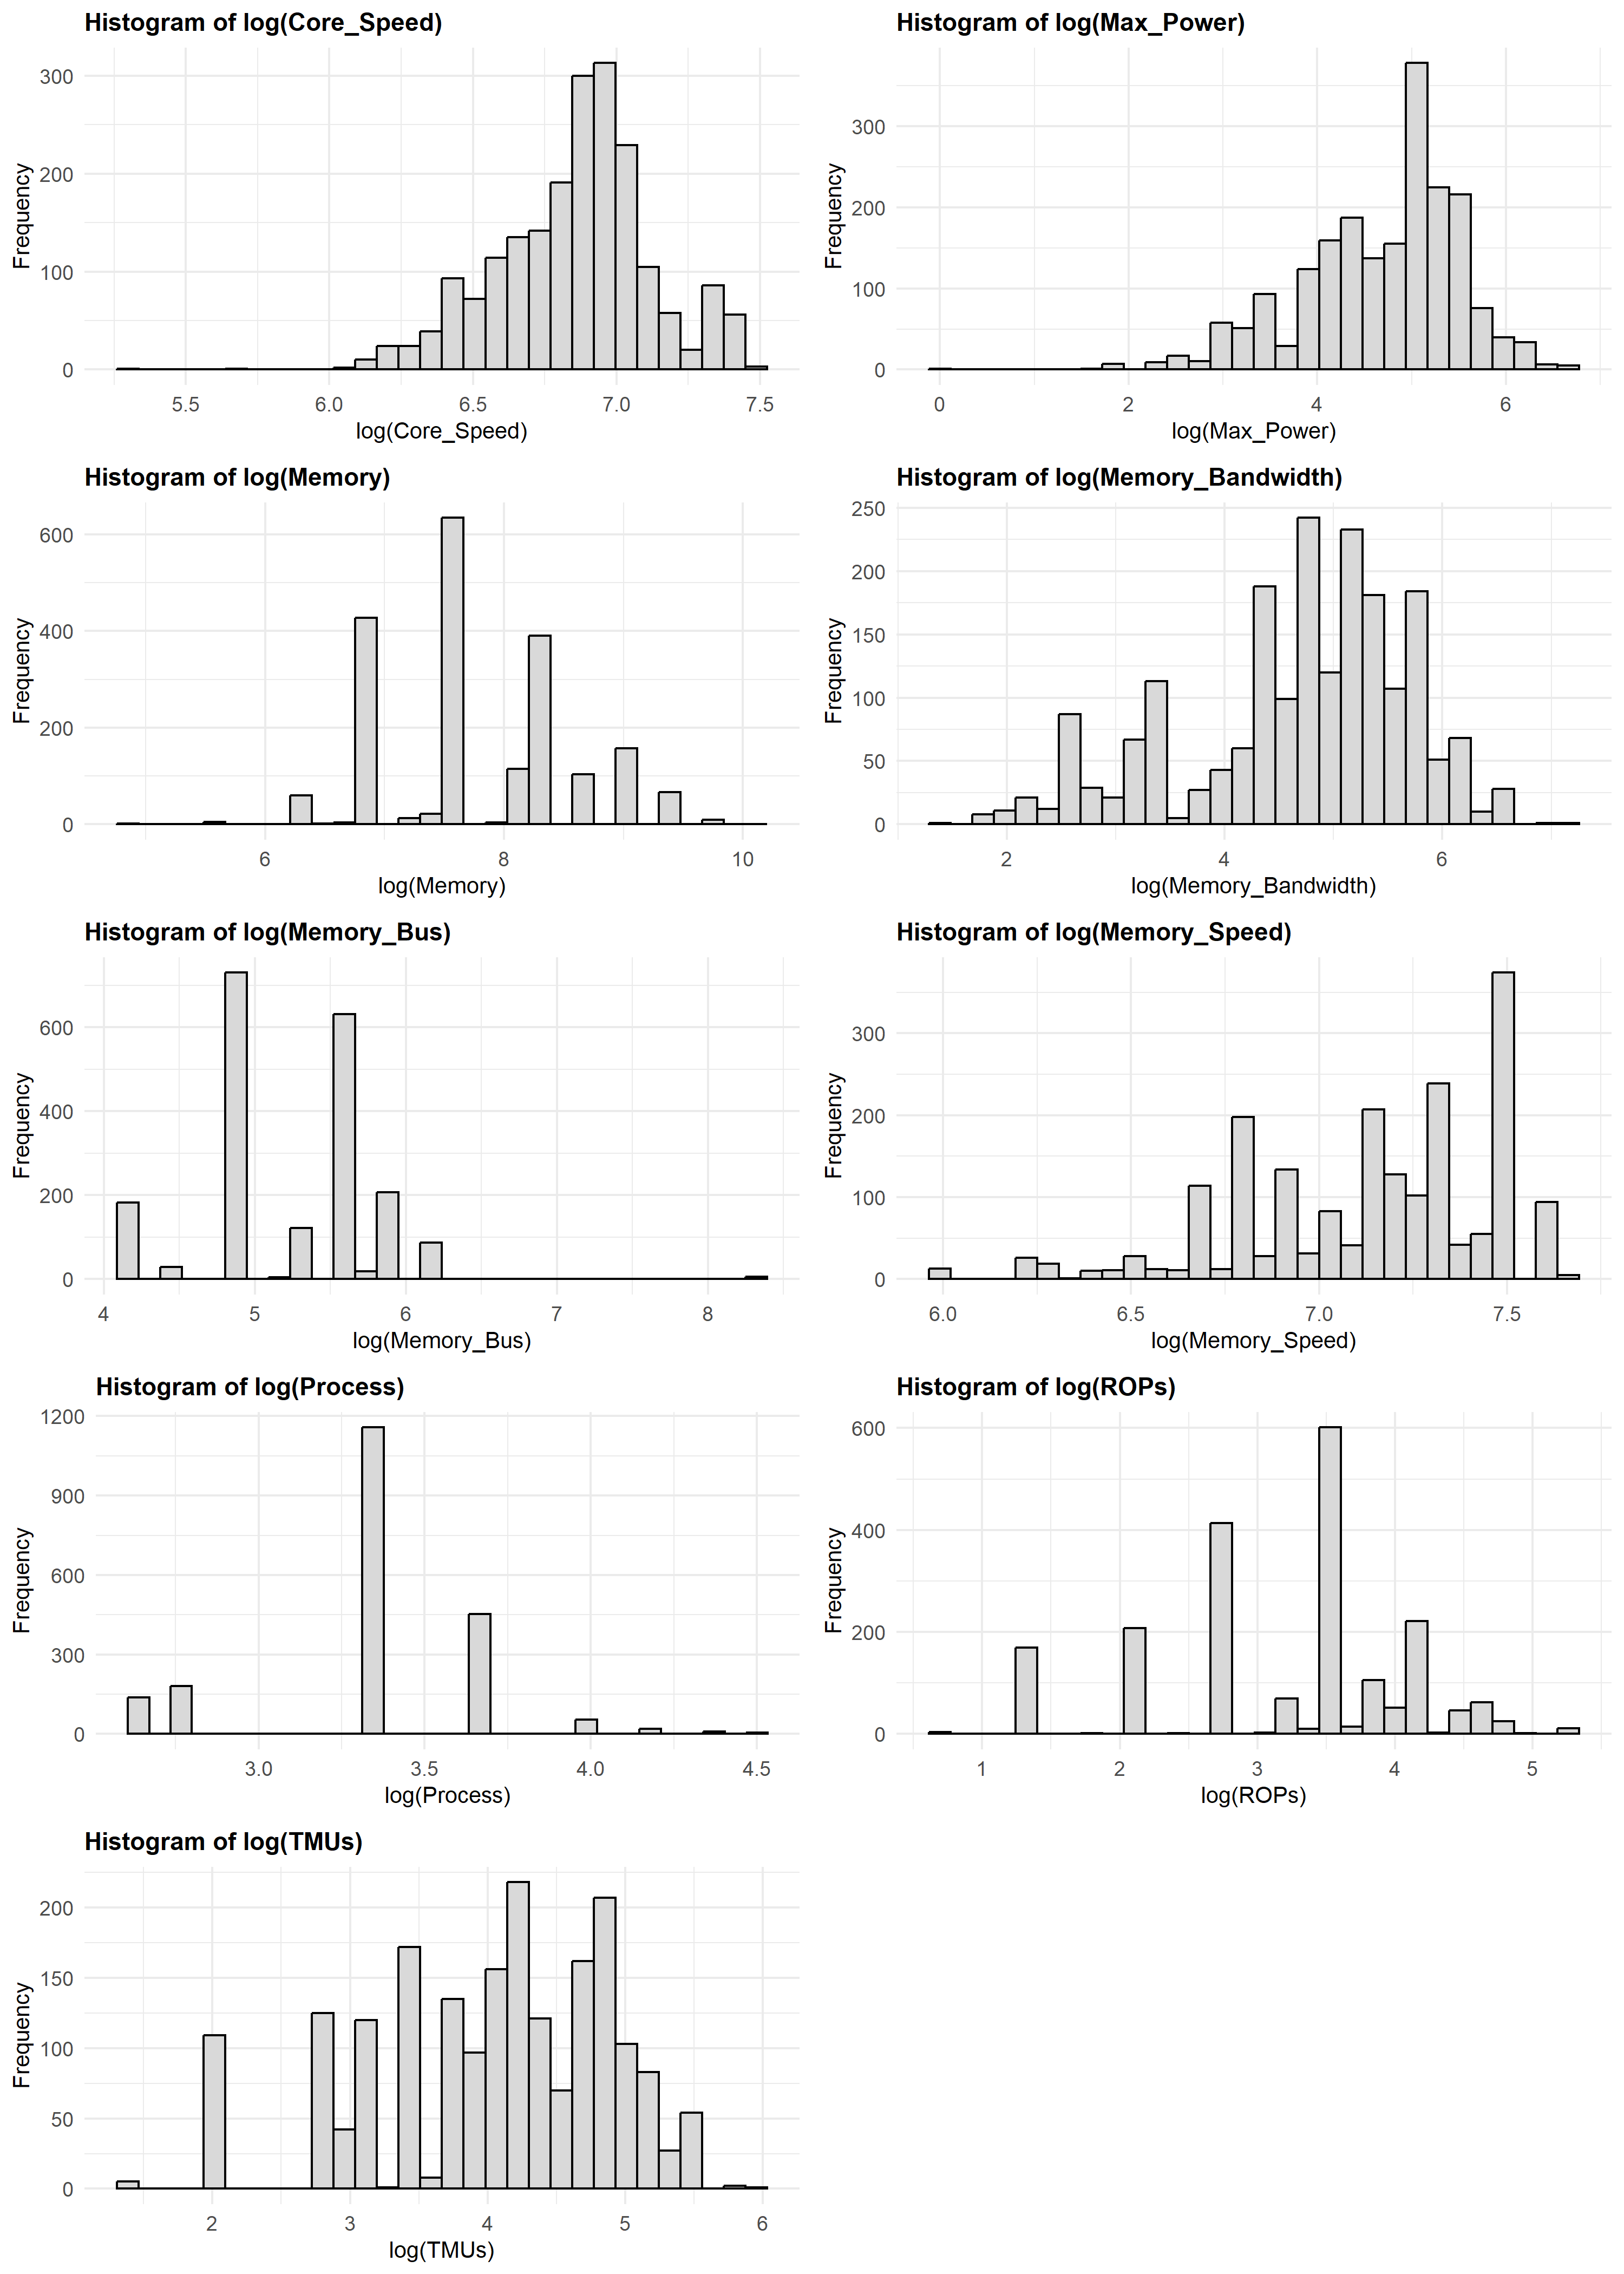
\includegraphics[width=0.92\textwidth]{statisticDes/histograms_log.png}
                \caption{Biểu đồ Histogram của các biến sau khi chuyển đổi sang dạng logarit}
                \label{fig:hist_log_r5}
            \end{figure}

            \textbf{Nhận xét về phân bố dữ liệu:}
            \begin{itemize}
                \item Ở dạng dữ liệu gốc (Hình \ref{fig:hist_original_r5}), hầu hết các biến phần cứng như \texttt{Memory}, \texttt{Memory\_Bandwidth}, \texttt{Max\_Power}, \texttt{ROPs}, và \texttt{TMUs} đều thể hiện độ lệch phải mạnh (Right-skewed distribution). Phần lớn các dòng GPU phổ thông tập trung ở khoảng giá trị nhỏ đến trung bình, trong khi một số ít GPU cao cấp nằm ở dải giá trị rất lớn.
                \item Sau khi áp dụng phép chuyển đổi logarit (Hình \ref{fig:hist_log_r5}), độ lệch của các biến được giảm đáng kể, phân bố dữ liệu trở nên đối xứng hơn và tiệm cận dạng phân phối chuẩn. Điều này giúp ổn định phương sai và đáp ứng tốt hơn các giả định của mô hình hồi quy tuyến tính ở các phần sau.
            \end{itemize}

        \subsubsection{Biểu đồ phân tán (Scatter Plot)}
            Để đánh giá mối quan hệ giữa biến phụ thuộc \texttt{log(Core\_Speed)} và các biến độc lập còn lại, nhóm tiến hành vẽ các biểu đồ phân tán dạng log bằng R:

            \begin{figure}[H]
                \centering
                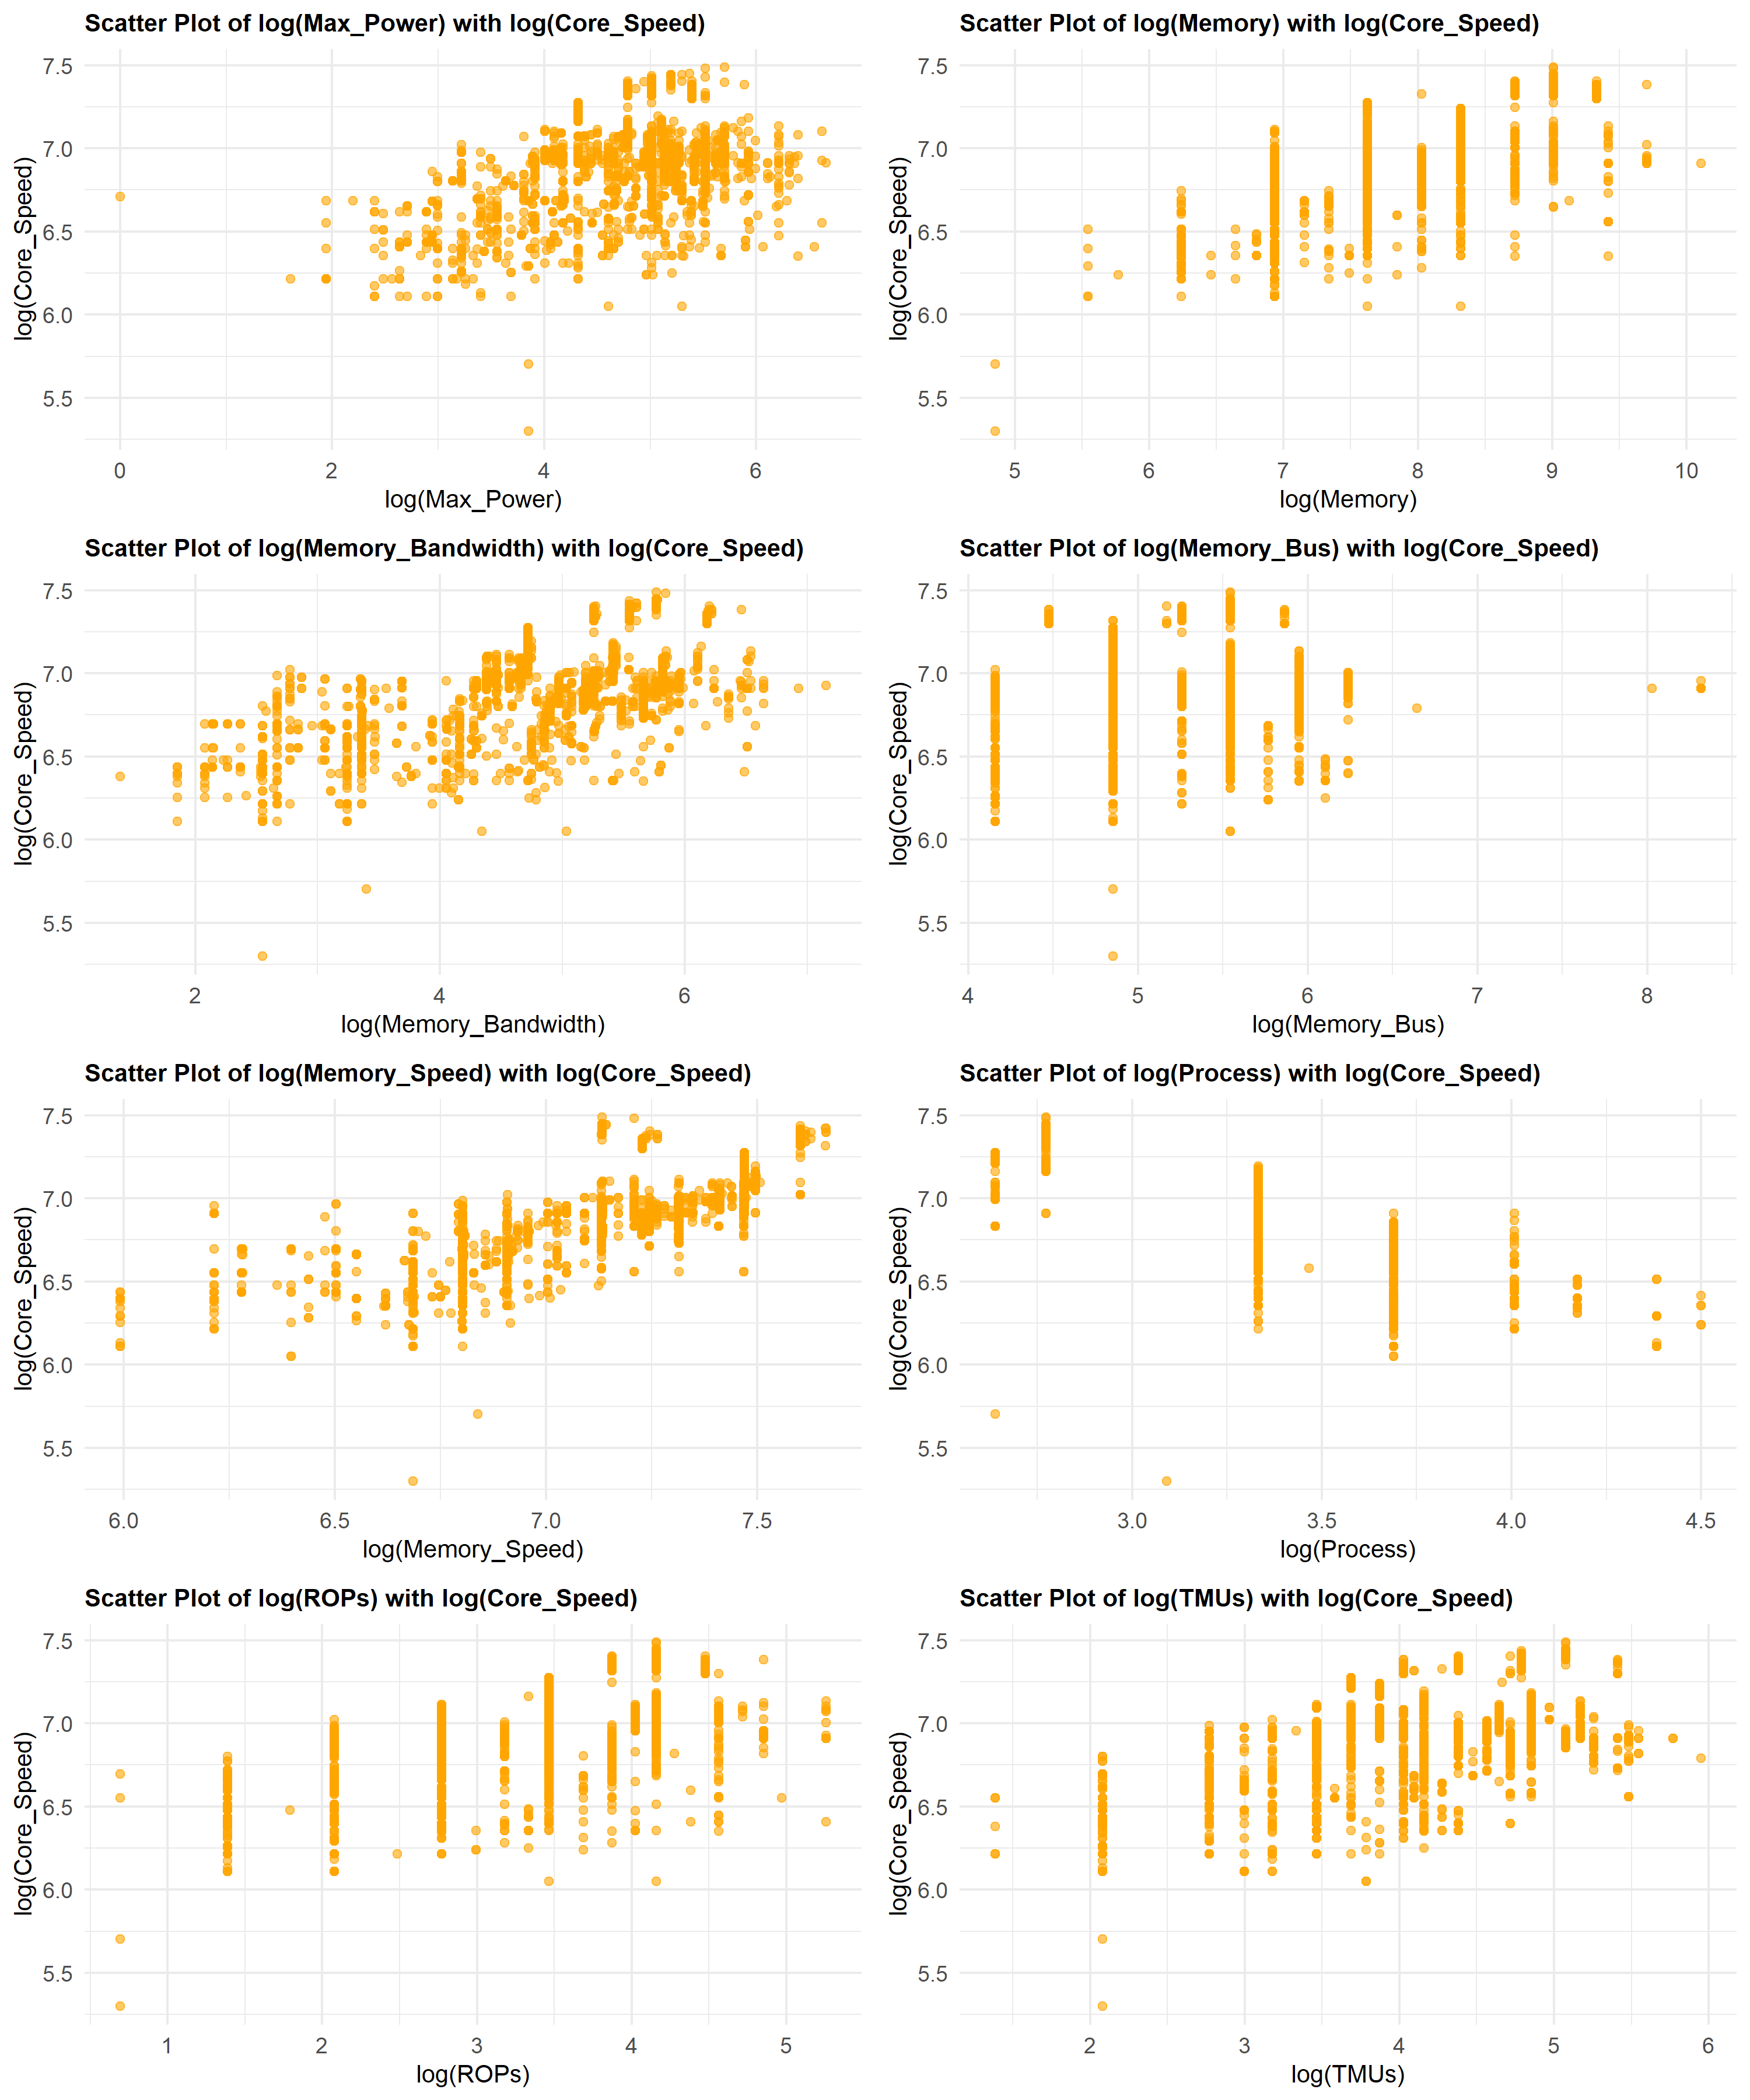
\includegraphics[width=0.92\textwidth]{statisticDes/scatter_log.png}
                \caption{Biểu đồ phân tán (Scatter Plot) giữa các biến độc lập với log(Core\_Speed)}
                \label{fig:scatter_log}
            \end{figure}

            \textbf{Nhận xét về mối quan hệ giữa các biến:}
            \begin{itemize}
                \item Dựa vào đồ thị phân tán giữa các biến \texttt{log(Max\_Power)}, \texttt{log(Memory\_Bandwidth)}, \texttt{log(Memory\_Speed)}, \texttt{log(Memory)}, \texttt{log(ROPs)}, \texttt{log(TMUs)} với \texttt{log(Core\_Speed)}, ta thấy mối quan hệ giữa các biến này với \texttt{log(Core\_Speed)} chủ yếu là \textbf{đồng biến} và phân tán với mật độ tương đối dày đặc.
                \item Đối với biến \texttt{log(Process)} (tiến trình sản xuất, nm), ta quan sát thấy xu hướng \textbf{nghịch biến} so với \texttt{log(Core\_Speed)}: công nghệ tiến trình nm càng nhỏ (bán dẫn càng tiên tiến) thì xung nhịp nhân \texttt{Core\_Speed} đạt được càng cao.
                \item Mối quan hệ dạng logarit thể hiện xu hướng tuyến tính rõ ràng hơn so với dữ liệu gốc, tạo tiền đề thuận lợi cho việc xây dựng mô hình hồi quy tuyến tính bội ở Phần 6.
            \end{itemize}
\newpage
\section{Thống kê suy diễn}
    \subsection{Phân tích phương sai một nhân tố (ANOVA) và hậu kiểm theo nhà sản xuất}
    \textbf{Bài toán:} Trên thị trường card đồ họa hiện nay, có 4 nhãn hàng chính cạnh tranh với nhau là \textbf{AMD}, \textbf{ATI}, \textbf{Intel} và \textbf{Nvidia}. Tốc độ xung nhịp nhân (\texttt{Core\_Speed}, đơn vị: MHz) là một trong những thông số cốt lõi phản ánh năng lực xử lý của GPU. Với mức ý nghĩa $\alpha = 0.05$, hãy đánh giá xem nhà sản xuất (\texttt{Manufacturer}) có ảnh hưởng đến tốc độ xung nhịp nhân trung bình của GPU hay không.

    \subsubsection{Thống kê mô tả và xây dựng giả thuyết}
        Sau khi chuẩn hóa dữ liệu và loại bỏ trùng lặp theo tên từng mẫu GPU (\texttt{Name}), bộ dữ liệu thu được $N = 2,469$ mẫu GPU thuộc 4 nhà sản xuất, trong đó cỡ mẫu của từng nhóm đều lớn hơn $30$ ($n_i \ge 80$), đảm bảo điều kiện áp dụng Định lý Giới hạn Trung tâm:

        \begin{table}[H]
            \centering
            \renewcommand{\arraystretch}{1.3}
            \begin{tabular}{|l|r|r|r|r|r|}
                \hline
                \textbf{Nhà sản xuất} & \textbf{Số lượng ($n$)} & \textbf{Trung bình (Mean)} & \textbf{Độ lệch chuẩn (SD)} & \textbf{Trung vị (Median)} & \textbf{IQR} \\
                \hline
                \texttt{AMD} & 852 & 896.41 & 166.57 & 925.00 & 218.00 \\
                \hline
                \texttt{ATI} & 80 & 1076.53 & 83.40 & 1120.00 & 30.00 \\
                \hline
                \texttt{Intel} & 115 & 355.05 & 153.24 & 300.00 & 50.00 \\
                \hline
                \texttt{Nvidia} & 1422 & 1017.59 & 276.57 & 1006.00 & 355.00 \\
                \hline
            \end{tabular}
            \caption{Thống kê mô tả biến \texttt{Core\_Speed} (MHz) theo từng nhà sản xuất}
            \label{tab:anova_desc}
        \end{table}

        Gọi $\mu_{\text{AMD}}, \mu_{\text{ATI}}, \mu_{\text{Intel}}, \mu_{\text{Nvidia}}$ lần lượt là tốc độ xung nhịp nhân trung bình của GPU thuộc 4 nhà sản xuất. Ta thiết lập cặp giả thuyết kiểm định:
        \begin{itemize}
            \item $H_0: \mu_{\text{AMD}} = \mu_{\text{ATI}} = \mu_{\text{Intel}} = \mu_{\text{Nvidia}}$ (Không có sự khác biệt về tốc độ xung nhịp nhân trung bình giữa các nhà sản xuất).
            \item $H_1:$ Tồn tại ít nhất hai nhà sản xuất có tốc độ xung nhịp nhân trung bình khác nhau.
        \end{itemize}

    \subsubsection{Kiểm tra các giả định của mô hình ANOVA}
        \begin{enumerate}
            \item \textbf{Tính độc lập của các quan sát:} Các mẫu GPU trong bộ dữ liệu đại diện cho từng dòng sản phẩm độc lập sau khi đã lọc trùng theo tên sản phẩm, do đó giả định độc lập được thỏa mãn.
            \item \textbf{Kiểm định phân phối chuẩn (Shapiro-Wilk Test):}
            \begin{itemize}
                \item Kết quả kiểm định Shapiro-Wilk trên cả 4 nhóm đều cho $\text{p-value} < 0.05$ ($\text{AMD}: W = 0.967, p = 6.14 \times 10^{-13}$; $\text{ATI}: W = 0.709, p = 2.70 \times 10^{-11}$; $\text{Intel}: W = 0.686, p = 2.35 \times 10^{-14}$; $\text{Nvidia}: W = 0.976, p = 1.71 \times 10^{-14}$).
                \item Tuy nhiên, vì kích thước mẫu của cả 4 nhóm đều lớn ($n_{\min} = 80 > 30$), theo Định lý Giới hạn Trung tâm, phân phối của trung bình mẫu tiệm cận phân phối chuẩn nên phương pháp ANOVA vẫn đảm bảo tính vững (robustness).
            \end{itemize}
            \item \textbf{Kiểm định tính đồng nhất phương sai (Levene's Test):}
            \begin{itemize}
                \item Giả thuyết $H_0$: Phương sai của \texttt{Core\_Speed} giữa 4 nhà sản xuất là bằng nhau ($\sigma_1^2 = \sigma_2^2 = \sigma_3^2 = \sigma_4^2$).
                \item Kết quả kiểm định Levene cho thống kê $F = 83.664$ với $\text{p-value} < 2.2 \times 10^{-16} < 0.05 \Rightarrow$ Bác bỏ $H_0$. Như vậy, phương sai giữa các nhóm là \textbf{không đồng nhất}.
                \item Để đảm bảo tính chính xác tuyệt đối khi giả định đồng nhất phương sai bị vi phạm, nhóm thực hiện song song cả \textbf{ANOVA tiêu chuẩn} và kiểm định hiệu chỉnh \textbf{Welch's ANOVA} (\texttt{oneway.test(..., var.equal = FALSE)}).
            \end{itemize}
        \end{enumerate}
        \begin{figure}[H]
            \centering
            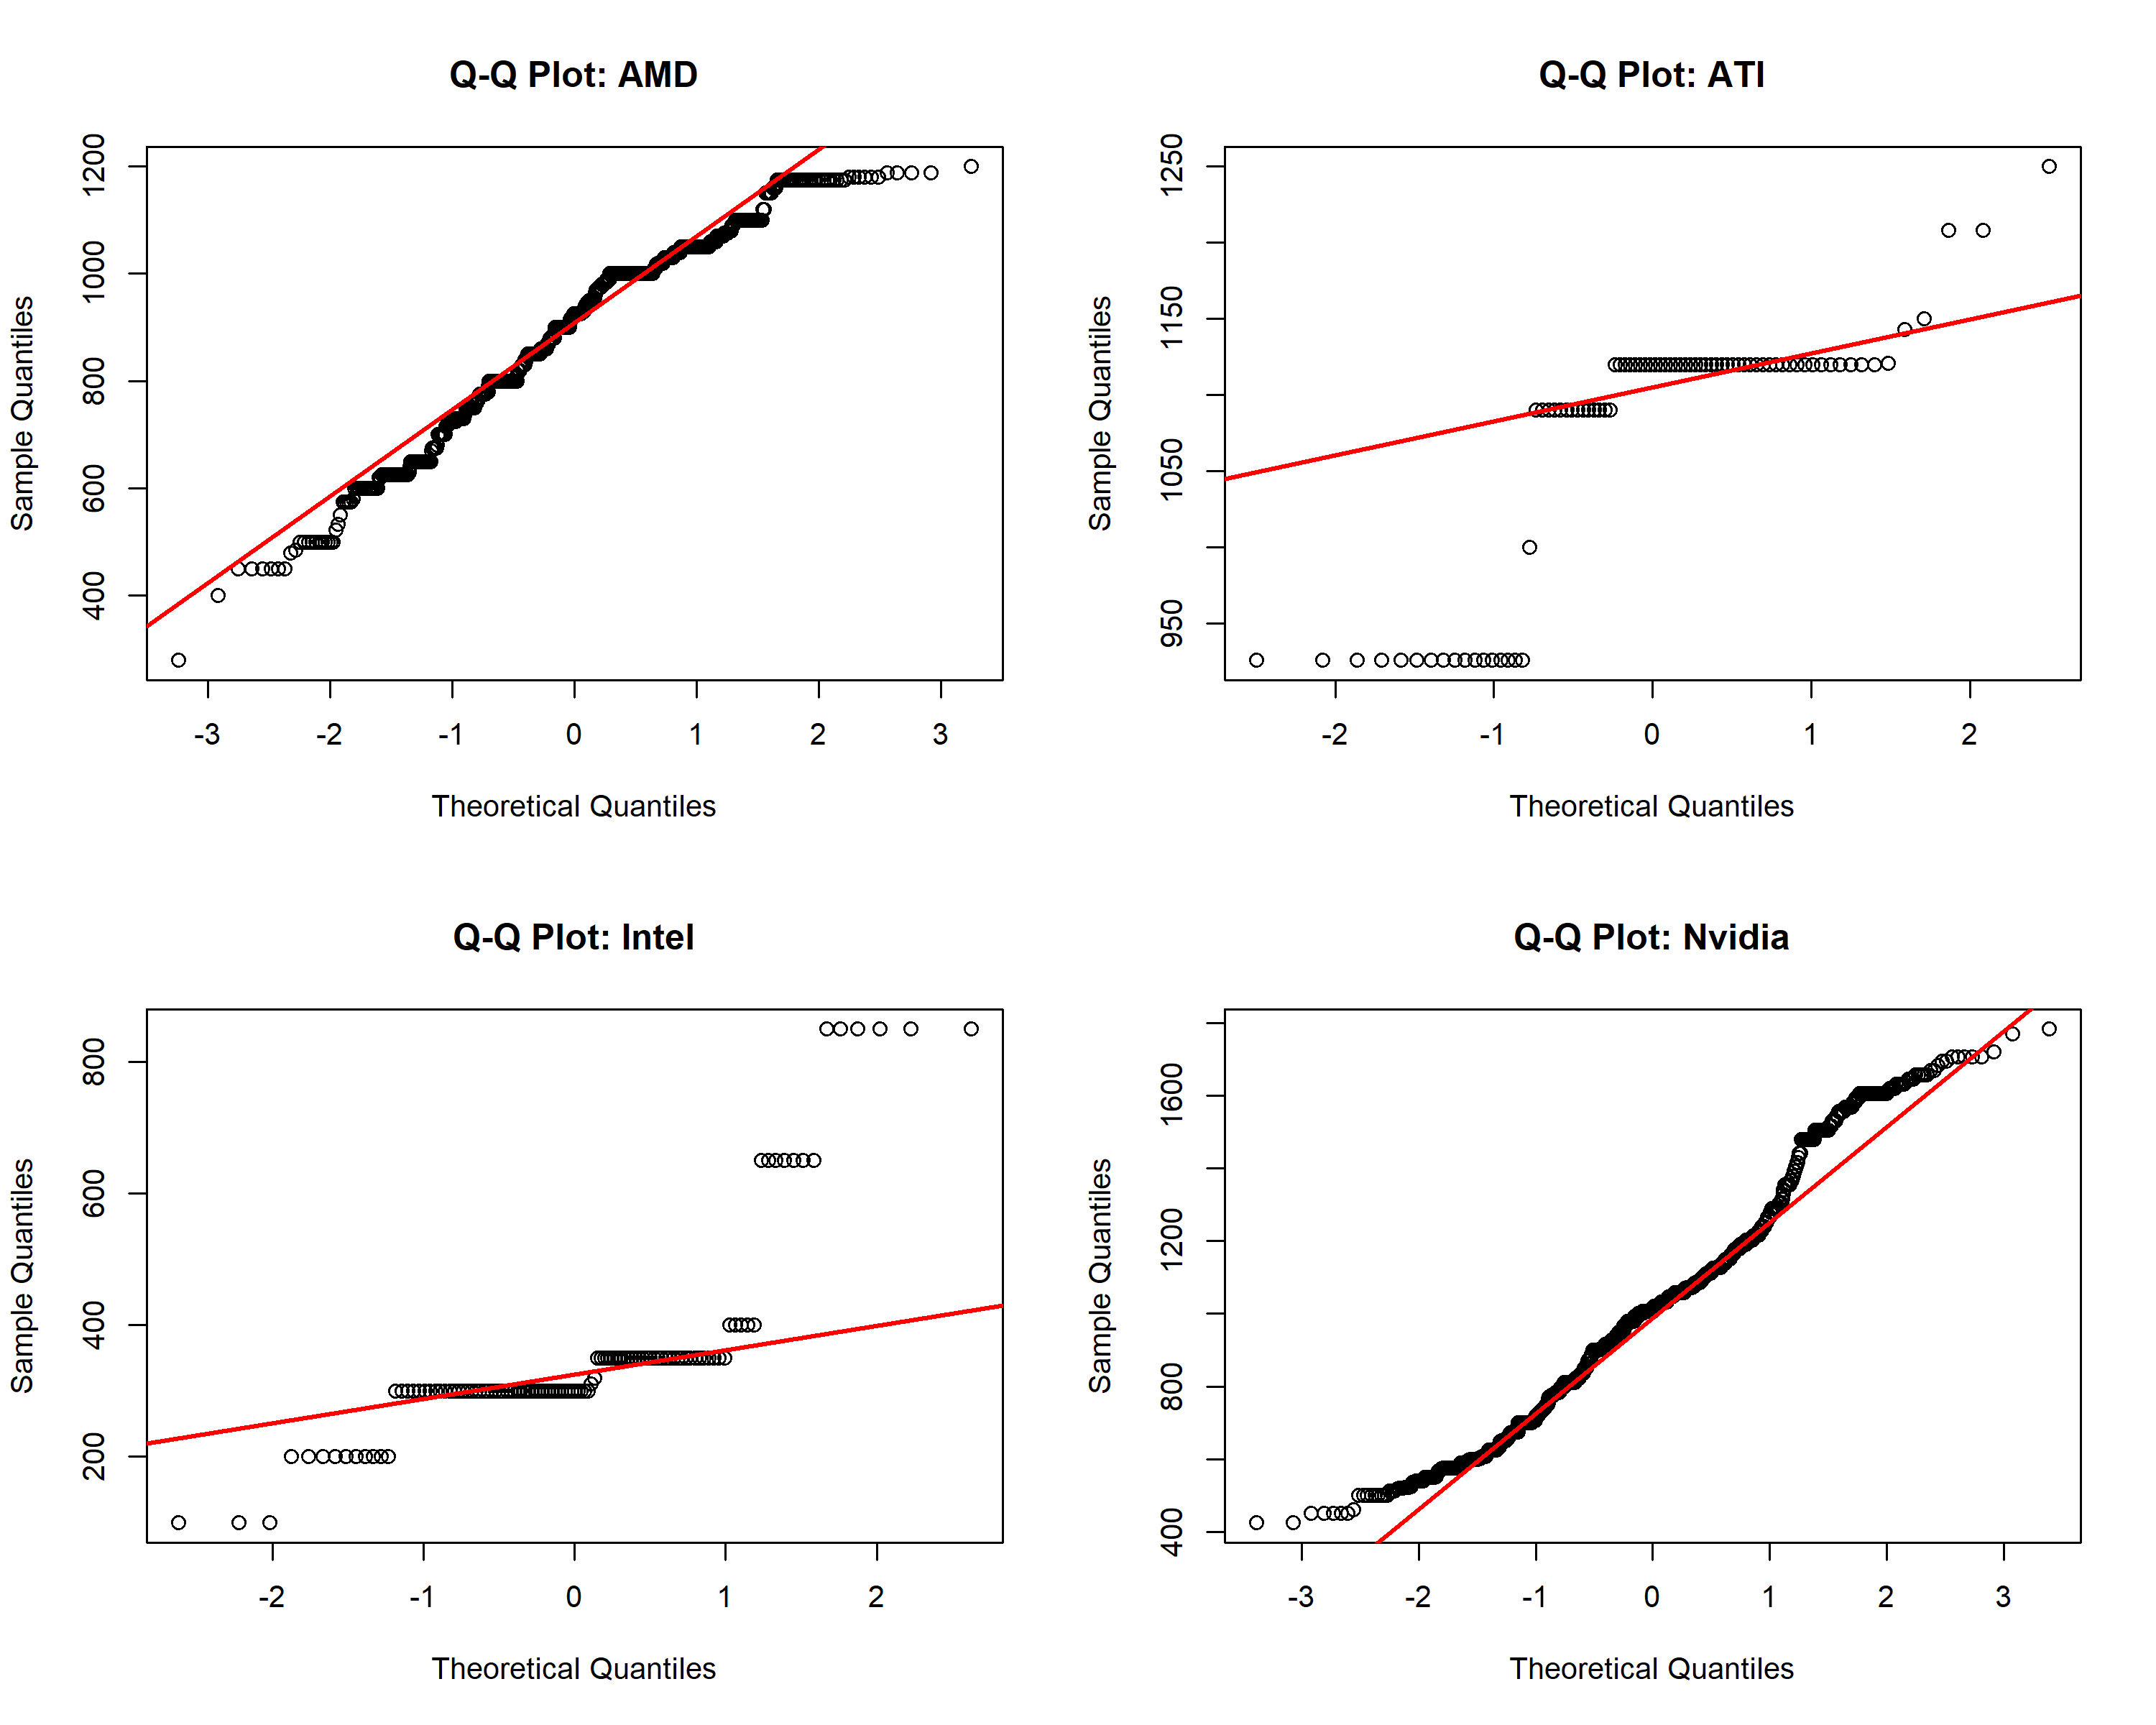
\includegraphics[width=0.9\textwidth]{statisticPros/anova_qqplot.png}
            \caption{Biểu đồ Q-Q Plot kiểm tra phân phối chuẩn của \texttt{Core\_Speed} theo 4 nhà sản xuất}
            \label{fig:anova_qqplot}
        \end{figure}
        
        \begin{figure}[H]
            \centering
            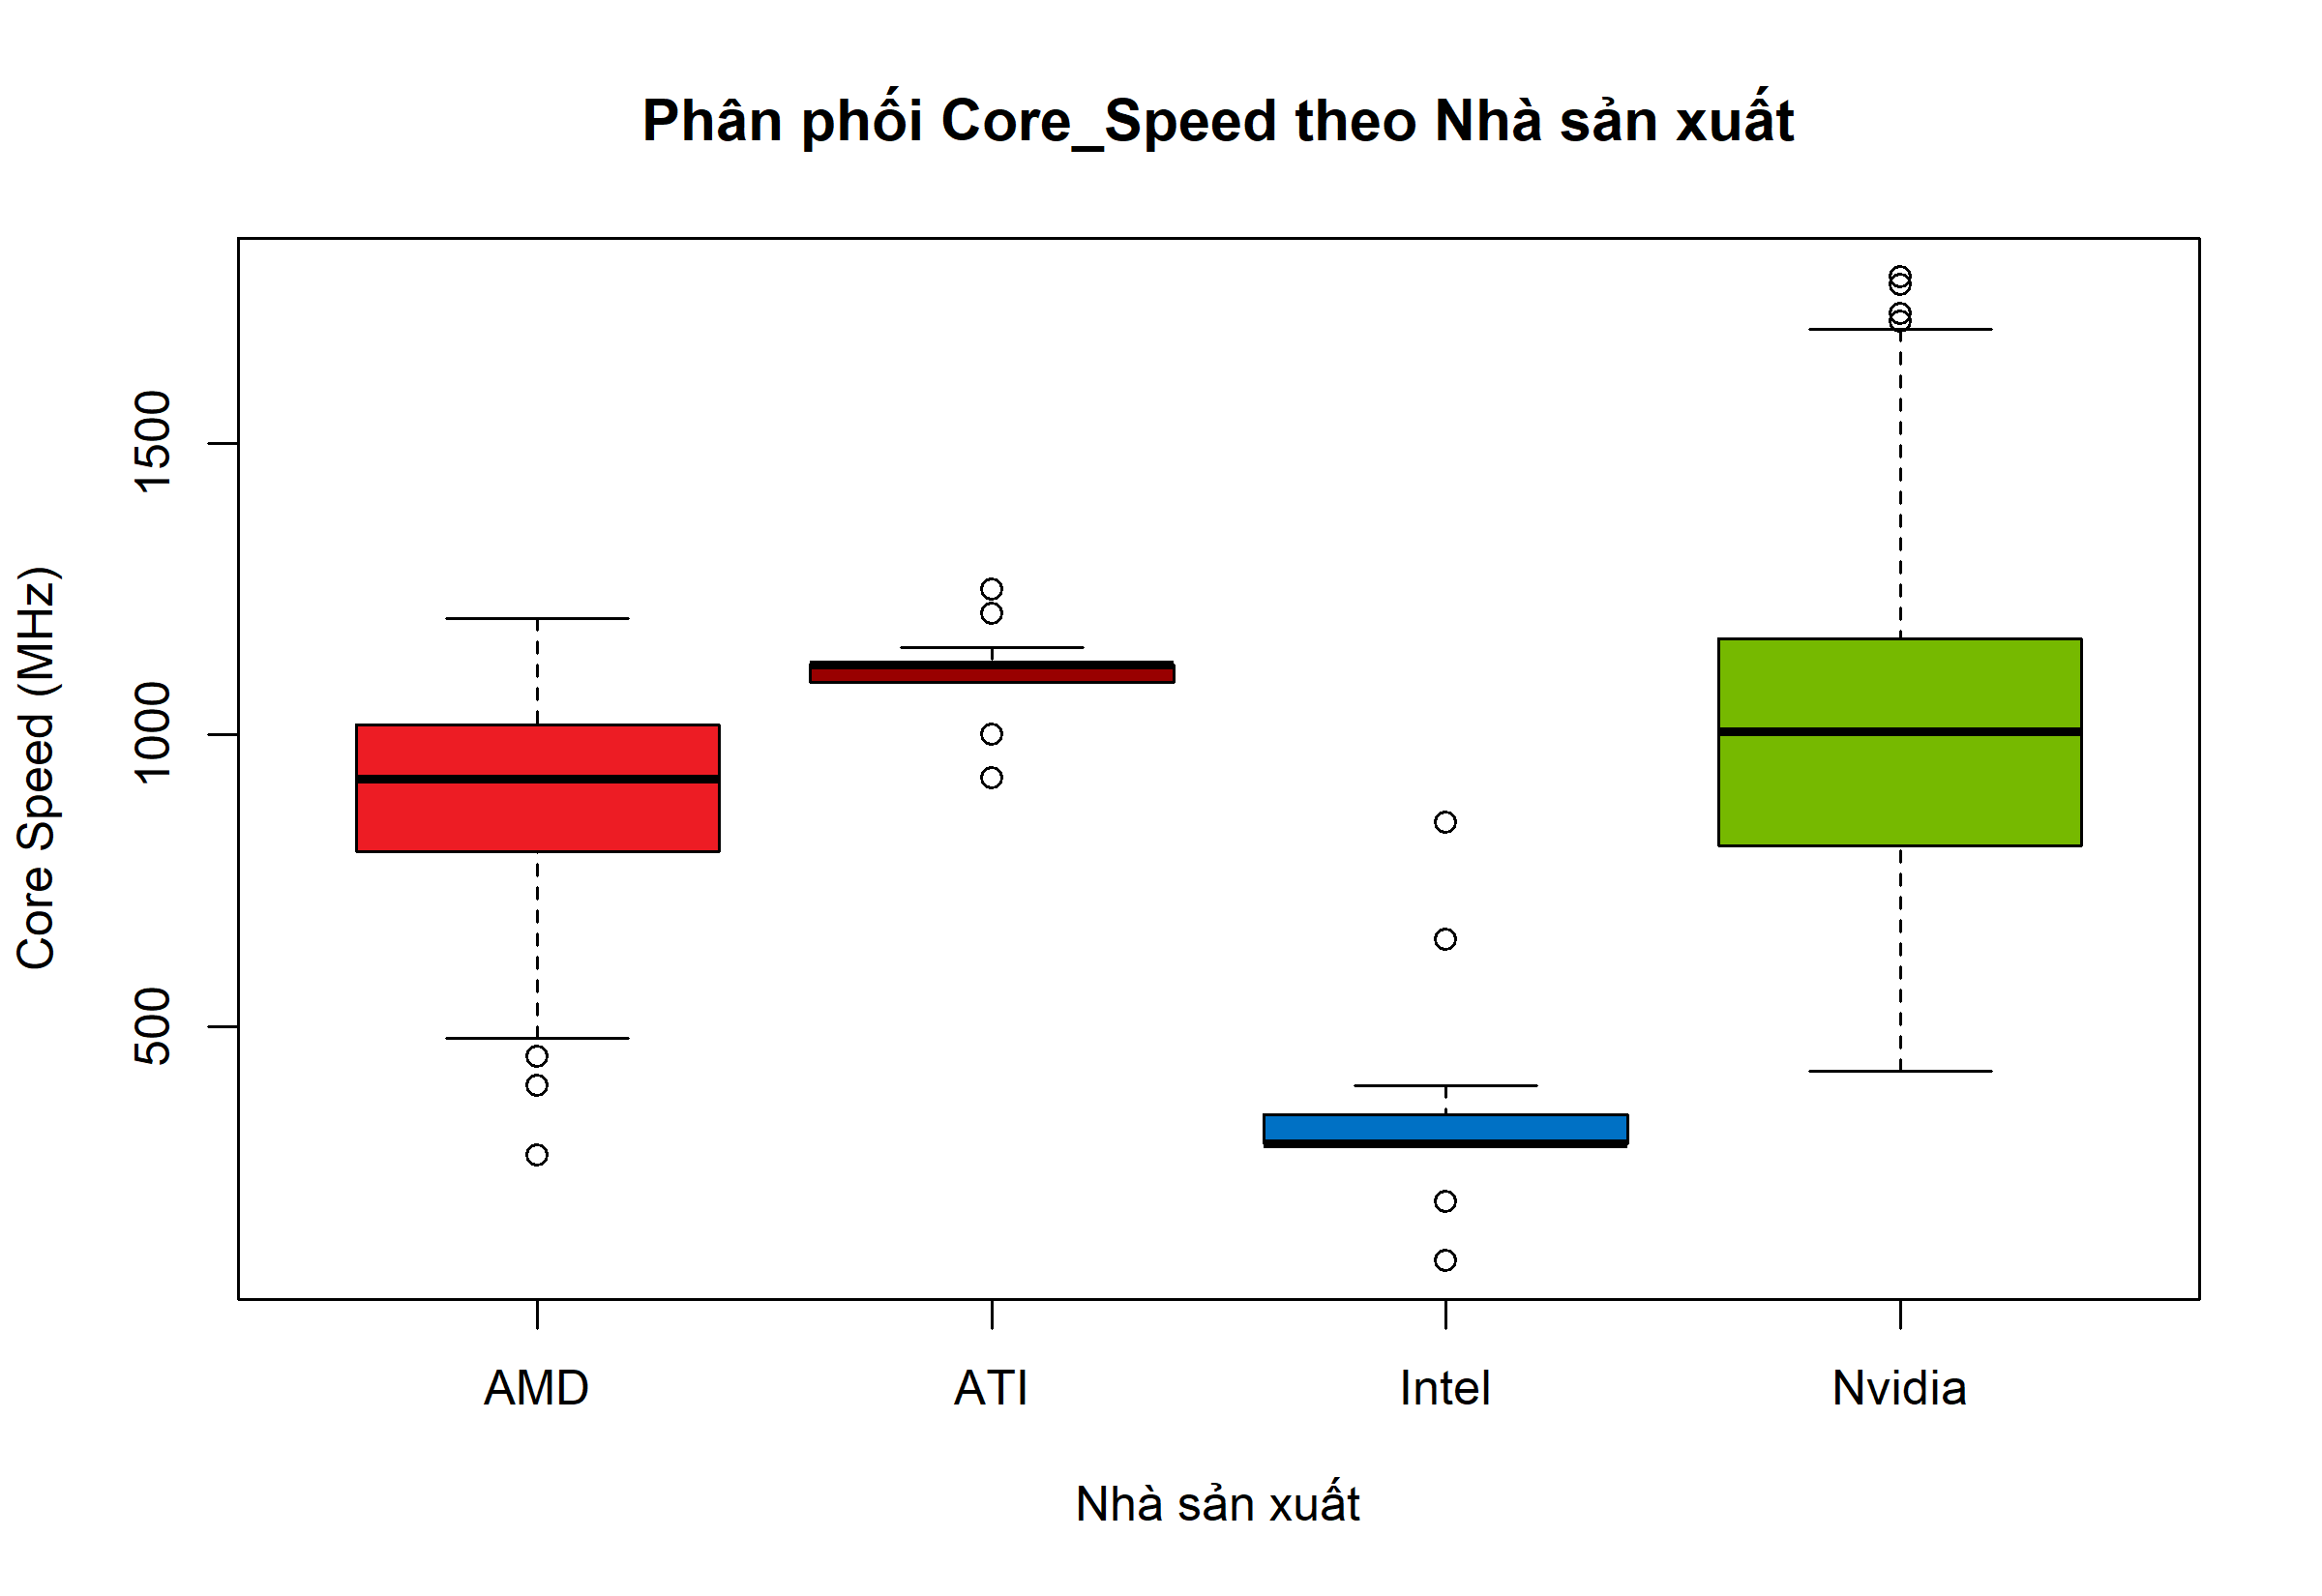
\includegraphics[width=0.82\textwidth]{statisticPros/anova_boxplot.png}
            \caption{Biểu đồ Boxplot so sánh phân phối \texttt{Core\_Speed} giữa các nhà sản xuất}
            \label{fig:anova_boxplot}
        \end{figure}


    \subsubsection{Kết quả mô hình ANOVA và phân tích hậu kiểm (Post-hoc)}
        \textbf{1. Kết quả kiểm định ANOVA:}
        \begin{itemize}
            \item \textbf{ANOVA tiêu chuẩn:} Thống kê $F(3, 2465) = 308.6$, $\text{p-value} < 2 \times 10^{-16} < \alpha = 0.05$.
            \item \textbf{Welch's ANOVA (không giả định phương sai bằng nhau):} Thống kê $F(3, 297.24) = 676.55$, $\text{p-value} < 2.2 \times 10^{-16} < \alpha = 0.05$.
            \item $\Rightarrow$ Cả hai phương pháp đều dẫn đến quyết định \textbf{bác bỏ $H_0$}. Có sự khác biệt có ý nghĩa thống kê rất cao về tốc độ xung nhịp nhân trung bình giữa các nhà sản xuất GPU.
        \end{itemize}

        \textbf{2. Phân tích hậu kiểm Tukey HSD (So sánh bội từng cặp):}
        \begin{table}[H]
            \centering
            \renewcommand{\arraystretch}{1.3}
            \begin{tabular}{|l|r|r|r|r|l|}
                \hline
                \textbf{Cặp so sánh} & \textbf{Chênh lệch (diff)} & \textbf{Cận dưới (lwr)} & \textbf{Cận trên (upr)} & \textbf{$p_{\text{adj}}$} & \textbf{Kết luận ($\alpha = 0.05$)} \\
                \hline
                \texttt{ATI - AMD} & $+180.11$ & $+109.62$ & $+250.60$ & $0.0000$ & Khác biệt có ý nghĩa \\
                \hline
                \texttt{Intel - AMD} & $-541.36$ & $-601.25$ & $-481.47$ & $0.0000$ & Khác biệt có ý nghĩa \\
                \hline
                \texttt{Nvidia - AMD} & $+121.17$ & $+95.06$ & $+147.29$ & $0.0000$ & Khác biệt có ý nghĩa \\
                \hline
                \texttt{Intel - ATI} & $-721.47$ & $-809.23$ & $-633.71$ & $0.0000$ & Khác biệt có ý nghĩa \\
                \hline
                \texttt{Nvidia - ATI} & $-58.94$ & $-128.21$ & $+10.33$ & $0.1269$ & \textbf{Không có sự khác biệt} \\
                \hline
                \texttt{Nvidia - Intel} & $+662.53$ & $+604.09$ & $+720.97$ & $0.0000$ & Khác biệt có ý nghĩa \\
                \hline
            \end{tabular}
            \caption{Kết quả kiểm định hậu kiểm Tukey HSD giữa các cặp nhà sản xuất}
            \label{tab:tukey_hsd}
        \end{table}

        \textbf{Kết luận rút ra từ mô hình ANOVA:}
        \begin{itemize}
            \item \textbf{Nhóm hiệu năng xung nhịp cao (\texttt{ATI} và \texttt{Nvidia}):} Hai hãng này dẫn đầu về tốc độ xung nhịp nhân trung bình (lần lượt là $1076.53\text{ MHz}$ và $1017.59\text{ MHz}$). Đặc biệt, phép kiểm định hậu kiểm cho thấy giữa \texttt{Nvidia} và \texttt{ATI} \textbf{không có sự khác biệt có ý nghĩa thống kê} về tốc độ xung nhịp trung bình ($p_{\text{adj}} = 0.1269 > 0.05$).
            \item \textbf{Nhóm tầm trung (\texttt{AMD}):} Có tốc độ xung nhịp trung bình đạt $896.41\text{ MHz}$, thấp hơn đáng kể so với \texttt{ATI} ($-180.11\text{ MHz}$) và \texttt{Nvidia} ($-121.17\text{ MHz}$).
            \item \textbf{Nhóm xung nhịp thấp (\texttt{Intel}):} Có tốc độ xung nhịp trung bình thấp nhất ($355.05\text{ MHz}$), chênh lệch rất lớn so với cả 3 hãng còn lại ($p_{\text{adj}} < 0.0001$). Điều này hoàn toàn phù hợp với thực tế công nghệ vì đa số GPU của Intel trong tập dữ liệu là chip đồ họa tích hợp (iGPU) tối ưu cho tiết kiệm điện năng, trong khi AMD, ATI và Nvidia tập trung vào dòng card đồ họa rời (dGPU) hiệu năng cao.
        \end{itemize}


    \subsection{Mô hình hồi quy tuyến tính}
        Phân tích hồi quy tuyến tính bội (Multiple Linear Regression) là phương pháp thống kê nhằm xác định mối quan hệ tuyến tính giữa một biến phụ thuộc $Y$ với nhiều biến độc lập $X_1, X_2, \dots, X_n$, từ đó dự đoán giá trị của $Y$ khi các biến độc lập thay đổi. Phương trình tổng quát có dạng:
        \[Y = w_0 + w_1X_1 + w_2X_2 + \dots + w_nX_n + \varepsilon\]
        Trong phương trình hồi quy tuyến tính đa biến có những yếu tố sau:
        \begin{itemize}
            \item $Y$: Biến phụ thuộc (giá trị đầu ra cần dự đoán của mô hình).
            \item $X_1, X_2, \dots, X_n$: Các biến độc lập (các biến đầu vào của mô hình).
            \item $w_0$: Hệ số chặn (Intercept).
            \item $w_1, w_2, \dots, w_n$: Các trọng số (hệ số hồi quy), thể hiện mức độ ảnh hưởng của từng biến đầu vào đến kết quả dự đoán.
            \item $\varepsilon$: Sai số ngẫu nhiên, thể hiện phần biến thiên của giá trị thực tế mà mô hình chưa giải thích được.
        \end{itemize}

    \subsection{Mục tiêu và phương pháp xây dựng mô hình}
        \subsubsection{Mô hình 1}
            Ở mô hình này, ta phân tích sự tác động của 7 yếu tố phần cứng gồm: \texttt{Memory\_Bandwidth}, \texttt{Memory}, \texttt{Memory\_Speed}, \texttt{Memory\_Bus}, \texttt{Process}, \texttt{ROPs}, \texttt{TMUs} lên \texttt{Core\_Speed} (chưa xét đến công suất tiêu thụ tối đa).
            \begin{itemize}
                \item \textbf{Biến phụ thuộc:} \texttt{Core\_Speed}
                \item \textbf{Biến độc lập:} \texttt{Memory\_Bandwidth}, \texttt{Memory}, \texttt{Memory\_Speed}, \texttt{Memory\_Bus}, \texttt{Process}, \texttt{ROPs}, \texttt{TMUs}
            \end{itemize}
            Phương trình biểu diễn mô hình:
            \[\texttt{Core\_Speed} = w_0 + w_1X_1 + w_2X_2 + \dots + w_7X_7 + \varepsilon\]

        \subsubsection{Mô hình 2}
            Mô hình 2 khảo sát sự tác động khi lược bỏ bớt biến tốc độ bộ nhớ (\texttt{Memory\_Speed}) và công suất (\texttt{Max\_Power}), giữ lại 6 biến độc lập: \texttt{Memory\_Bandwidth}, \texttt{Memory}, \texttt{Memory\_Bus}, \texttt{Process}, \texttt{ROPs}, \texttt{TMUs}.
            \begin{itemize}
                \item \textbf{Biến phụ thuộc:} \texttt{Core\_Speed}
                \item \textbf{Biến độc lập:} \texttt{Memory\_Bandwidth}, \texttt{Memory}, \texttt{Memory\_Bus}, \texttt{Process}, \texttt{ROPs}, \texttt{TMUs}
            \end{itemize}

        \subsubsection{Mô hình 3 (Mô hình dạng Logarit đầy đủ)}
            Ở mô hình chính này, ta áp dụng phép biến đổi logarit tự nhiên ($\ln$) cho toàn bộ biến phụ thuộc và đầy đủ 8 biến độc lập để tuyến tính hóa mối quan hệ và ổn định phương sai:
            \begin{itemize}
                \item \textbf{Biến phụ thuộc:} $\log(\texttt{Core\_Speed})$
                \item \textbf{Biến độc lập:} $\log(\texttt{Max\_Power})$, $\log(\texttt{Memory\_Bandwidth})$, $\log(\texttt{Memory})$, $\log(\texttt{Memory\_Speed})$, $\log(\texttt{Memory\_Bus})$, $\log(\texttt{Process})$, $\log(\texttt{ROPs})$, $\log(\texttt{TMUs})$
            \end{itemize}

            \textbf{Mã nguồn R xây dựng và tóm tắt Mô hình 3:}
\begin{pythoncode}
Model3 <- lm(Core_Speed ~ Max_Power + Memory_Bandwidth + Memory + Memory_Speed + 
               Memory_Bus + Process + ROPs + TMUs, data = df_log)
print(summary(Model3))
\end{pythoncode}

            \begin{figure}[H]
                \centering
                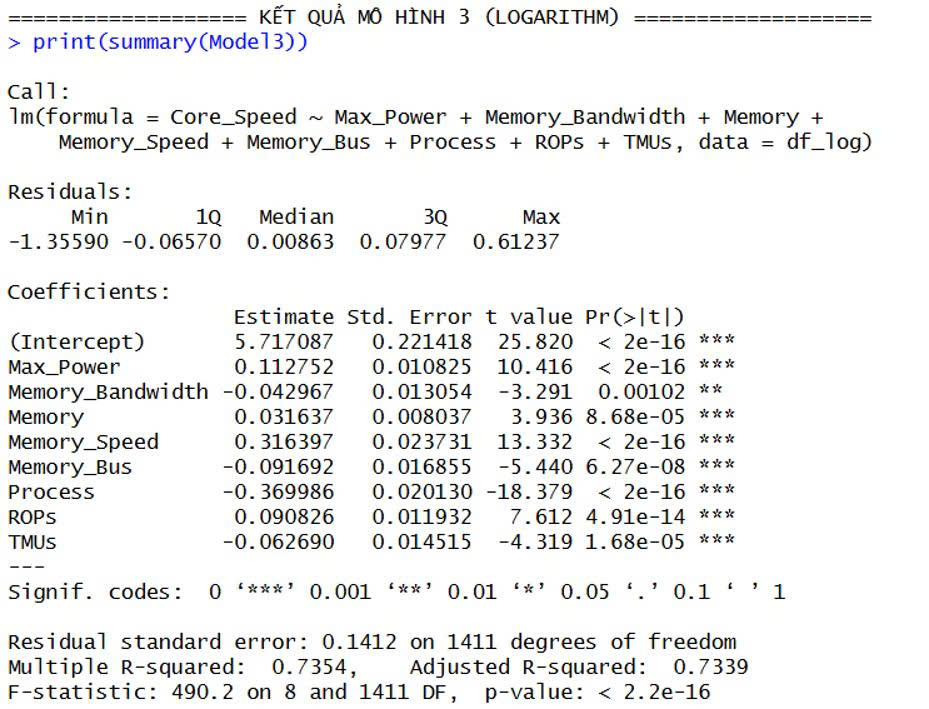
\includegraphics[width=0.92\textwidth]{statisticPros/model3_summary.jpg}
                \caption{Kết quả hồi quy tuyến tính bội của Mô hình 3 trong R}
                \label{fig:model3_summary}
            \end{figure}

    \subsection{Phân tích sự tác động của các yếu tố lên hiệu năng GPUs}
        Từ bảng kết quả ước lượng của Mô hình 3 (Hình \ref{fig:model3_summary}), phương trình hồi quy tuyến tính biểu diễn ảnh hưởng của các nhân tố đến xung nhịp nhân \texttt{Core\_Speed} của GPU có dạng:
        \begin{align*}
            \log(\texttt{Core\_Speed}) &= 5.717087 + 0.112752 \times \log(\texttt{Max\_Power}) - 0.042967 \times \log(\texttt{Memory\_Bandwidth}) \\
            &\quad + 0.031637 \times \log(\texttt{Memory}) + 0.316397 \times \log(\texttt{Memory\_Speed}) \\
            &\quad - 0.091692 \times \log(\texttt{Memory\_Bus}) - 0.369986 \times \log(\texttt{Process}) \\
            &\quad + 0.090826 \times \log(\texttt{ROPs}) - 0.062690 \times \log(\texttt{TMUs})
        \end{align*}

        \textbf{Đánh giá chi tiết mô hình:}
        \begin{itemize}
            \item \textbf{Kiểm định sự phù hợp chung (F-test):} Giá trị thống kê $F = 490.2$ (với bậc tự do $8$ và $1411$) có giá trị $\text{p-value} < 2.2 \times 10^{-16}$, nhỏ hơn rất nhiều so với mức ý nghĩa $\alpha = 0.05$ (thậm chí nhỏ hơn mức $0.001$). Điều này chứng tỏ mô hình hồi quy xây dựng được là rất phù hợp và các biến độc lập có ý nghĩa giải thích rất cao cho biến phụ thuộc \texttt{Core\_Speed}.
            \item \textbf{Đánh giá ý nghĩa thống kê của từng biến độc lập (t-test):} Xét cột trọng số (\texttt{Estimate}) và giá trị $\text{p-value}$ ($\Pr(>\vert{}t\vert{})$) tương ứng, tất cả 8 biến độc lập đều có $\text{p-value}$ rất nhỏ:
            \begin{itemize}
                \item Biến \texttt{Memory\_Bandwidth} có $\text{p-value} = 0.00102$ (đạt mức ý nghĩa $0.01$ — ký hiệu \texttt{**}).
                \item 7 biến còn lại (\texttt{Max\_Power}, \texttt{Memory}, \texttt{Memory\_Speed}, \texttt{Memory\_Bus}, \texttt{Process}, \texttt{ROPs}, \texttt{TMUs}) đều có $\text{p-value} < 0.0001$ (đạt mức ý nghĩa cực kỳ cao $0.001$ — ký hiệu \texttt{***}).
                \item $\Rightarrow$ Như vậy, cả 8 nhân tố đưa vào mô hình đều có ý nghĩa thống kê rất cao và thực sự tác động đến tốc độ xung nhịp \texttt{Core\_Speed} của GPUs.
            \end{itemize}
            \item \textbf{Mức độ giải thích của mô hình ($R^2$):} Hệ số $R^2$ hiệu chỉnh (\texttt{Adjusted R-squared}) bằng $0.7339$ (và \texttt{Multiple R-squared} bằng $0.7354$), nghĩa là các biến độc lập trong mô hình giải thích được \textbf{73.39\%} sự biến thiên của hiệu năng \texttt{Core\_Speed}.
            \item \textbf{Kết luận chiều hướng tác động:} Qua dấu của các trọng số thu được từ mô hình, ta thấy có sự phân hóa rõ rệt giữa hai nhóm nhân tố:
            \begin{itemize}
                \item \textit{Nhóm tác động đồng biến (hệ số dương):} \texttt{Max\_Power} ($+0.112752$), \texttt{Memory} ($+0.031637$), \texttt{Memory\_Speed} ($+0.316397$) và \texttt{ROPs} ($+0.090826$) — khi các thông số này tăng thì \texttt{Core\_Speed} có xu hướng tăng theo.
                \item \textit{Nhóm tác động nghịch biến (hệ số âm):} \texttt{Memory\_Bandwidth} ($-0.042967$), \texttt{Memory\_Bus} ($-0.091692$), \texttt{Process} ($-0.369986$) và \texttt{TMUs} ($-0.062690$). Đặc biệt biến tiến trình sản xuất (\texttt{Process}) có tác động nghịch biến mạnh nhất, phản ánh đúng thực tế công nghệ rằng tiến trình bán dẫn càng thu nhỏ (số nm giảm) thì xung nhịp nhân GPU càng đạt hiệu năng cao hơn.
            \end{itemize}
        \end{itemize}

    \subsection{Đồ thị biểu thị sai số hồi quy}
        Để kiểm tra các giả định của mô hình hồi quy tuyến tính (tính tuyến tính, kỳ vọng sai số bằng 0, phân phối chuẩn của phần dư và phương sai đồng nhất), nhóm tiến hành phân tích 4 biểu đồ chẩn đoán phần dư:

        \subsubsection{Biểu đồ Residuals vs Fitted (Giá trị dư theo giá trị dự đoán)}
            \begin{figure}[H]
                \centering
                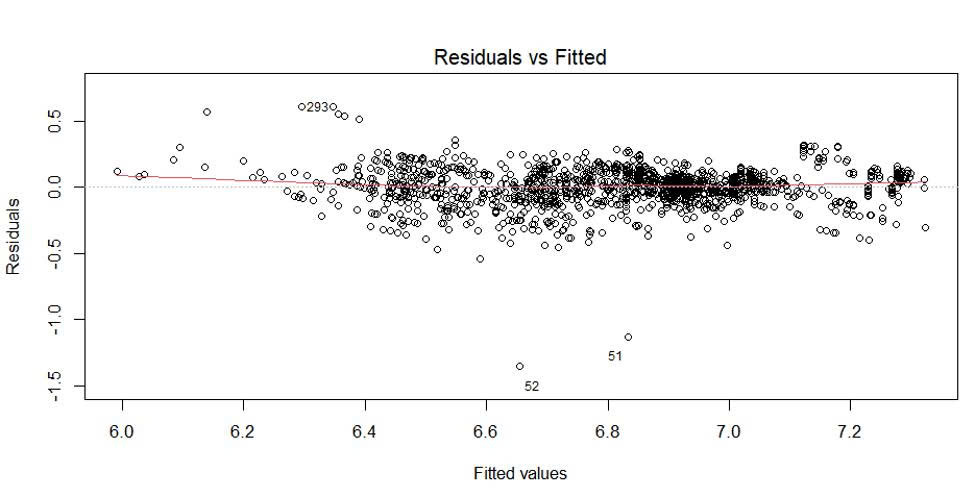
\includegraphics[width=0.88\textwidth]{statisticPros/diag_1_residuals_fitted.jpg}
                \caption{Biểu đồ Residuals vs Fitted}
                \label{fig:res_fitted}
            \end{figure}
            \textbf{Nhận xét:} Đường trung bình (đường màu đỏ) tương đối thẳng, nằm ngang và bám rất sát đường đứt nét $\text{Residuals} = 0$ xuyên suốt miền giá trị dự đoán. Điều này chứng tỏ giả thiết về tính tuyến tính của mô hình và giả thiết kỳ vọng của sai số bằng $0$ đều được thỏa mãn. Các điểm phần dư phân bố ngẫu nhiên quanh đường $0$ và chỉ xuất hiện một vài điểm ngoại lai nhỏ (như điểm 51, 52, 293) không làm ảnh hưởng đến xu hướng chung.

        \subsubsection{Biểu đồ Q-Q Residuals (Kiểm tra phân phối chuẩn)}
            \begin{figure}[H]
                \centering
                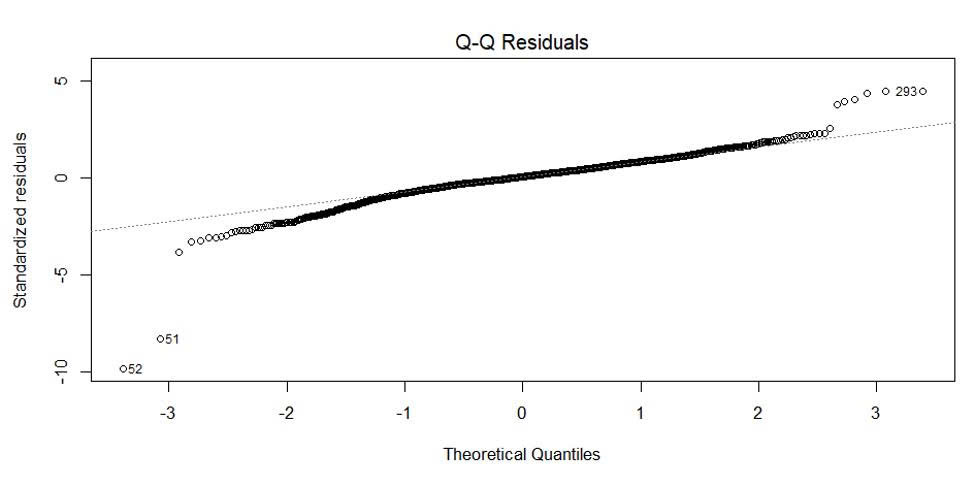
\includegraphics[width=0.88\textwidth]{statisticPros/diag_2_qq.jpg}
                \caption{Biểu đồ Q-Q Residuals}
                \label{fig:qq_res}
            \end{figure}
            \textbf{Nhận xét:} Đa số các điểm phần dư chuẩn hóa nằm bám sát đường thẳng chéo đứt nét trong khoảng giữa (từ $-1.5$ đến $+2.5$), cho thấy phần dư của mô hình nhìn chung tuân theo phân phối chuẩn. Tuy nhiên, ở hai đầu mút vẫn có một số điểm ngoại lai lệch hẳn khỏi đường chuẩn (như điểm 51, 52 lệch xuống dưới ở đuôi trái và điểm 293 lệch lên trên ở đuôi phải), tạo hiện tượng đuôi nặng nhẹ nhưng không làm ảnh hưởng lớn đến tính hợp lệ chung của mô hình do cỡ mẫu lớn.

        \subsubsection{Biểu đồ Scale-Location (Kiểm tra phương sai đồng nhất)}
            \begin{figure}[H]
                \centering
                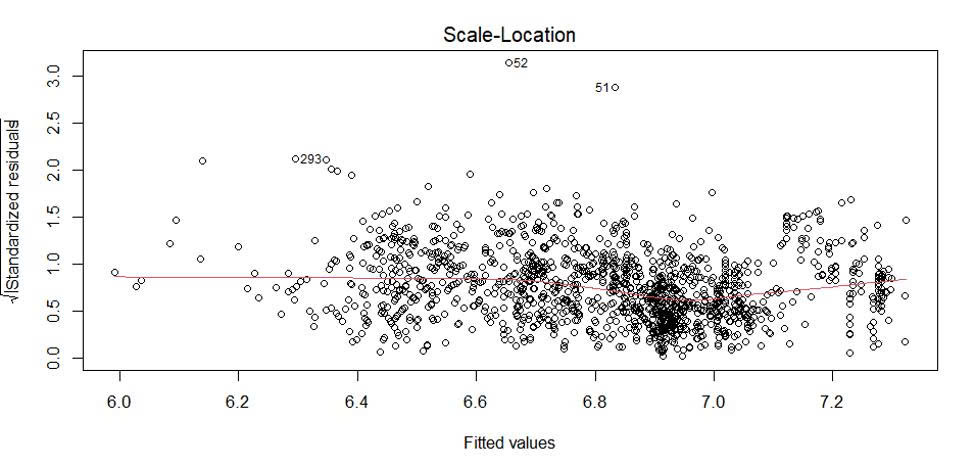
\includegraphics[width=0.88\textwidth]{statisticPros/diag_3_scale_location.jpg}
                \caption{Biểu đồ Scale-Location}
                \label{fig:scale_loc}
            \end{figure}
            \textbf{Nhận xét:} Đường xu hướng màu đỏ tương đối nằm ngang, dao động nhẹ quanh mức $0.6 - 0.85$ và các điểm dữ liệu phân bố khá đều trong dải từ $0.0$ đến $1.5$, không tạo thành hình phễu mở rộng hay thu hẹp rõ rệt dọc theo trục \texttt{Fitted values}. Điều này chứng tỏ giả thiết về phương sai đồng nhất của sai số (\textit{homoscedasticity}) cơ bản được thỏa mãn, chỉ xuất hiện một vài điểm ngoại lai có độ phân tán lớn như điểm 51, 52 và 293.

        \subsubsection{Biểu đồ Residuals vs Leverage (Giá trị dư theo đòn bẩy)}
            \begin{figure}[H]
                \centering
                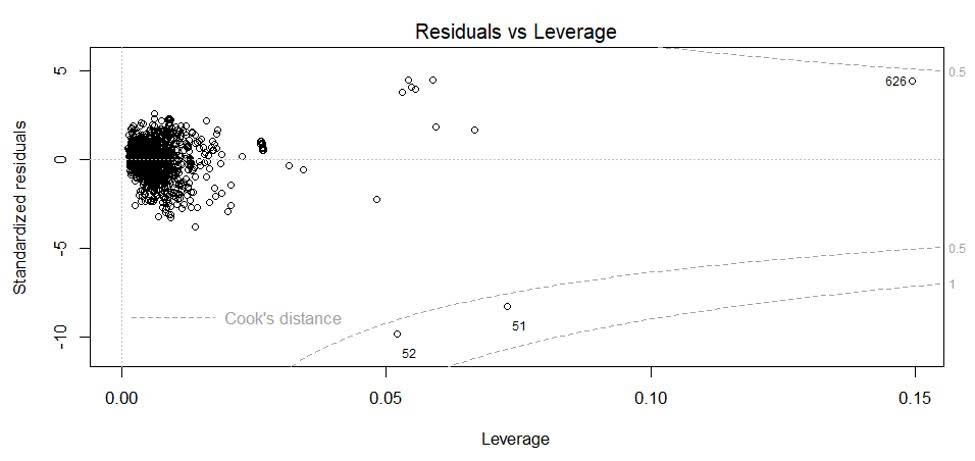
\includegraphics[width=0.88\textwidth]{statisticPros/diag_4_leverage.jpg}
                \caption{Biểu đồ Residuals vs Leverage}
                \label{fig:res_leverage}
            \end{figure}
            \textbf{Nhận xét:} Phần lớn các quan sát tập trung dày đặc ở vùng đòn bẩy thấp ($\text{Leverage} < 0.03$) và nằm hoàn toàn bên trong giới hạn khoảng cách Cook ($\text{Cook's distance} < 0.5$). Đồ thị phát hiện một số điểm có độ ảnh hưởng lớn là điểm 51 và 52 vượt ra ngoài đường giới hạn $0.5$ (nằm sát đường $1$), cùng điểm 626 có giá trị đòn bẩy cao ($\text{Leverage} \approx 0.15$) nhưng vẫn nằm dưới ngưỡng $0.5$. Nhìn chung, không có điểm nào vượt qua ngưỡng nguy hiểm ($\text{Cook's distance} > 1$), chứng tỏ mô hình khá ổn định và không bị bóp méo nghiêm trọng bởi các điểm ngoại lai.

    \subsection{Dự đoán giá trị dựa vào mô hình hồi quy}
        Sử dụng hàm \texttt{predict()} trên Mô hình 3 để tính toán giá trị xung nhịp dự đoán (cả ở dạng logarit và quy đổi ngược về đơn vị thực tế MHz qua hàm mũ $e^x$) và đối chiếu với dữ liệu thực tế:

        \begin{figure}[H]
            \centering
            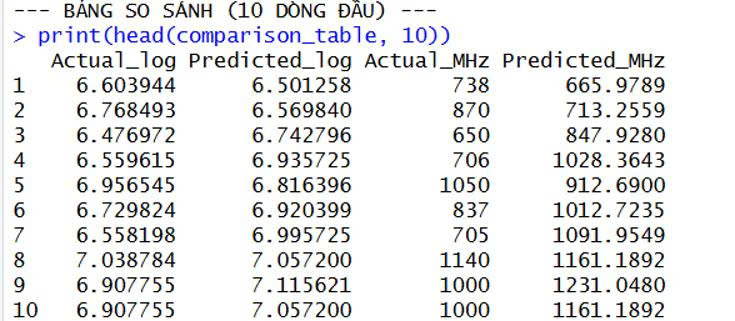
\includegraphics[width=0.85\textwidth]{statisticPros/predict_table.jpg}
            \caption{Bảng so sánh giá trị thực tế và giá trị dự đoán từ Mô hình 3 (10 quan sát đầu)}
            \label{fig:predict_table}
        \end{figure}

        \begin{figure}[H]
            \centering
            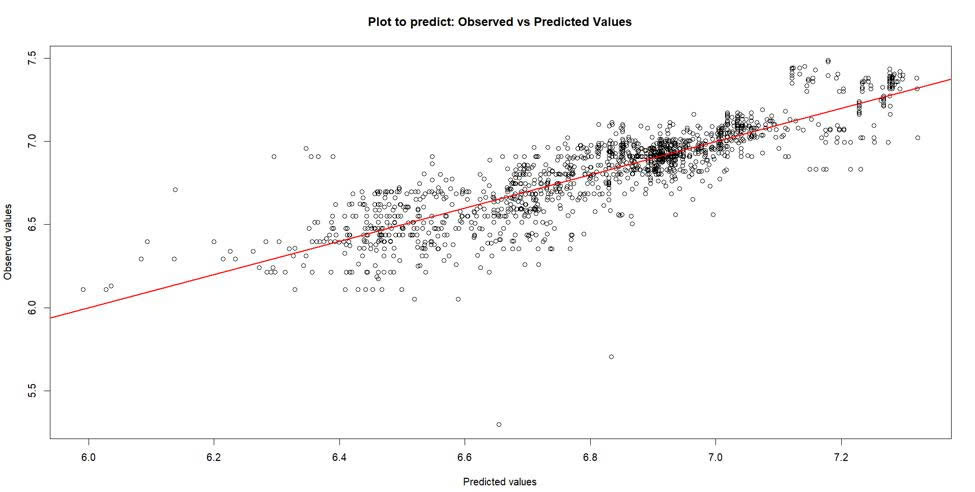
\includegraphics[width=0.88\textwidth]{statisticPros/plot_to_predict.jpg}
            \caption{Đồ thị so sánh giá trị dự đoán (Predicted) và giá trị thực tế (Observed)}
            \label{fig:plot_predict}
        \end{figure}

        \textbf{Đánh giá kết quả dự đoán:} Qua bảng so sánh số liệu (Hình \ref{fig:predict_table}) và đồ thị tương quan dự đoán (Hình \ref{fig:plot_predict}), các điểm quan sát bám khá sát đường xu hướng tuyến tính màu đỏ. Mặc dù mô hình chưa thể tái tạo chính xác tuyệt đối mọi giá trị thực tế, nhưng mức độ sai số nằm trong giới hạn nhỏ và hoàn toàn có thể chấp nhận được. Điều này khẳng định mô hình có độ tin cậy tốt và mang ý nghĩa thống kê cao.
\newpage
\section{Thảo luận và mở rộng}
\newpage
\section{Nguồn dữ liệu và nguồn code}
\newpage
%-------------------- main --------------------%

\phantomsection
% \addcontentsline{toc}{section}{Tài liệu tham khảo}
% \renewcommand{\refname}{Tài liệu tham khảo}
\nocite{*}
\bibliographystyle{apalike}
\bibliography{reference}

\end{document}